\documentclass[a4paper, titlepage]{article}

\usepackage[english]{babel}
\usepackage[utf8x]{inputenc}
\usepackage{amsmath}
\usepackage{amsfonts}
\usepackage{amssymb}
\usepackage{graphicx}
\usepackage{fullpage}
\usepackage{parskip}
\usepackage{setspace}
\usepackage[justification=centering]{caption}
\usepackage{subcaption}

\linespread{1.1}

\title{Visualisation AppStore \\ \vspace{10pt}
\textit{\large Integrated platform for visualistion submission, scheduling and visualisation wall playout} \\ \vspace*{-5pt}
\textit{\large Commissioned by Imperial Data Science Institute}}

\author{Andrew Higginson\\ Bryan Liu \\ Emma Hulme \\ Jia Guang Choo \\
        Thomas Taylor-Hall \\ Timothy van Bremen \\\\ 
        Department of Computing \\ Imperial College London \\\\ \textit{Supervised by:} \\
        Prof. Yi-ke Guo \\ Dr. David Birch}

\date{January 2015}

\begin{document}
\maketitle


\newpage
\pagenumbering{roman}
% -- Executive Summary
\Large
\textbf{Executive Summary}

\normalsize




% ---

\newpage
% -- Table of Contents
\tableofcontents
\listoffigures
\listoftables
% ---


\newpage
\pagenumbering{arabic}
\section{Introduction}
As part of the renovation of the William Penney Building, the part of the building facing onto the Sherfield walkway will be undergoing major changes in order to further promote the home of the Imperial Data Science Institute. These changes include mounting an 84 inch 4K touch panel adjacent to the building's entrance, as well as replacing the existing small windows with floor to ceiling glass panel, onto which content can be projected to the hundreds of students, teaching staff and visitors who pass by everyday.

\begin{figure}[h!]
\centering
\begin{subfigure}{.5\textwidth}
  \centering
  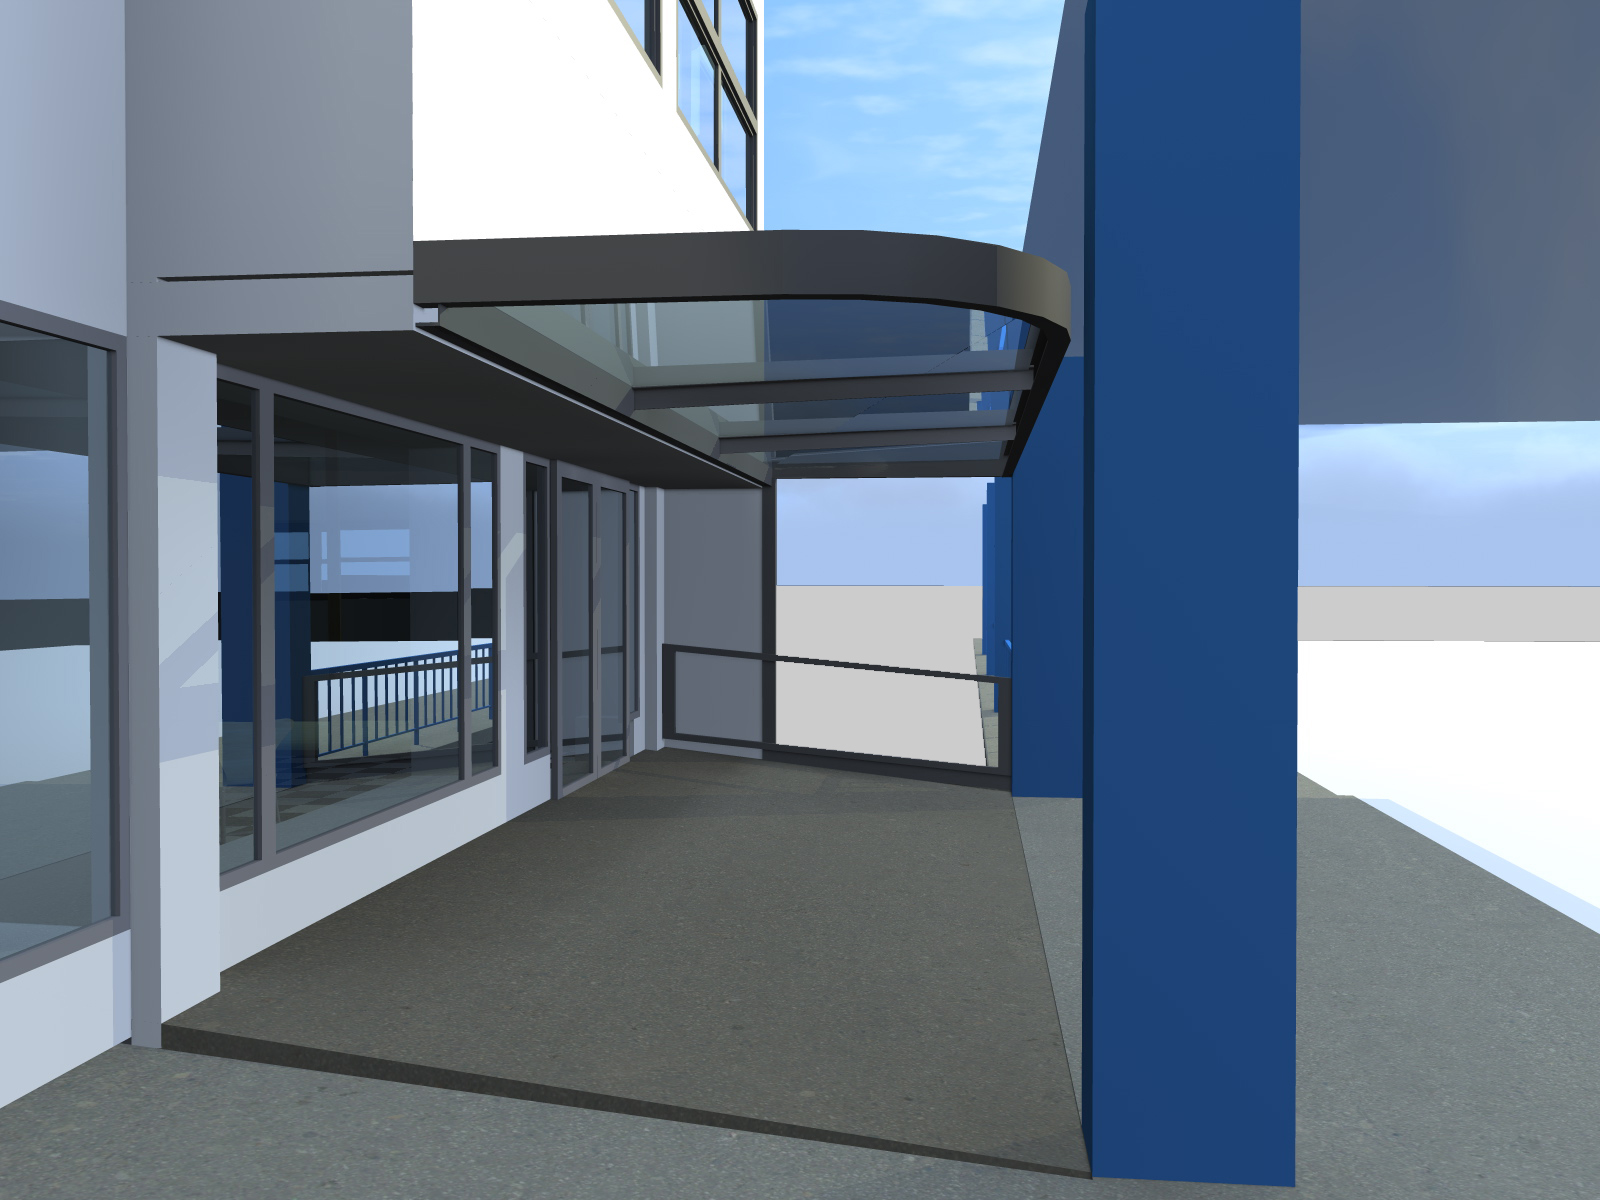
\includegraphics[width=.8\linewidth]{./intro/Entrance.jpg}
  \caption{A render of the proposed changes to the entrance}
  \label{fig:sub1}
\end{subfigure}%
\begin{subfigure}{.5\textwidth}
  \centering
  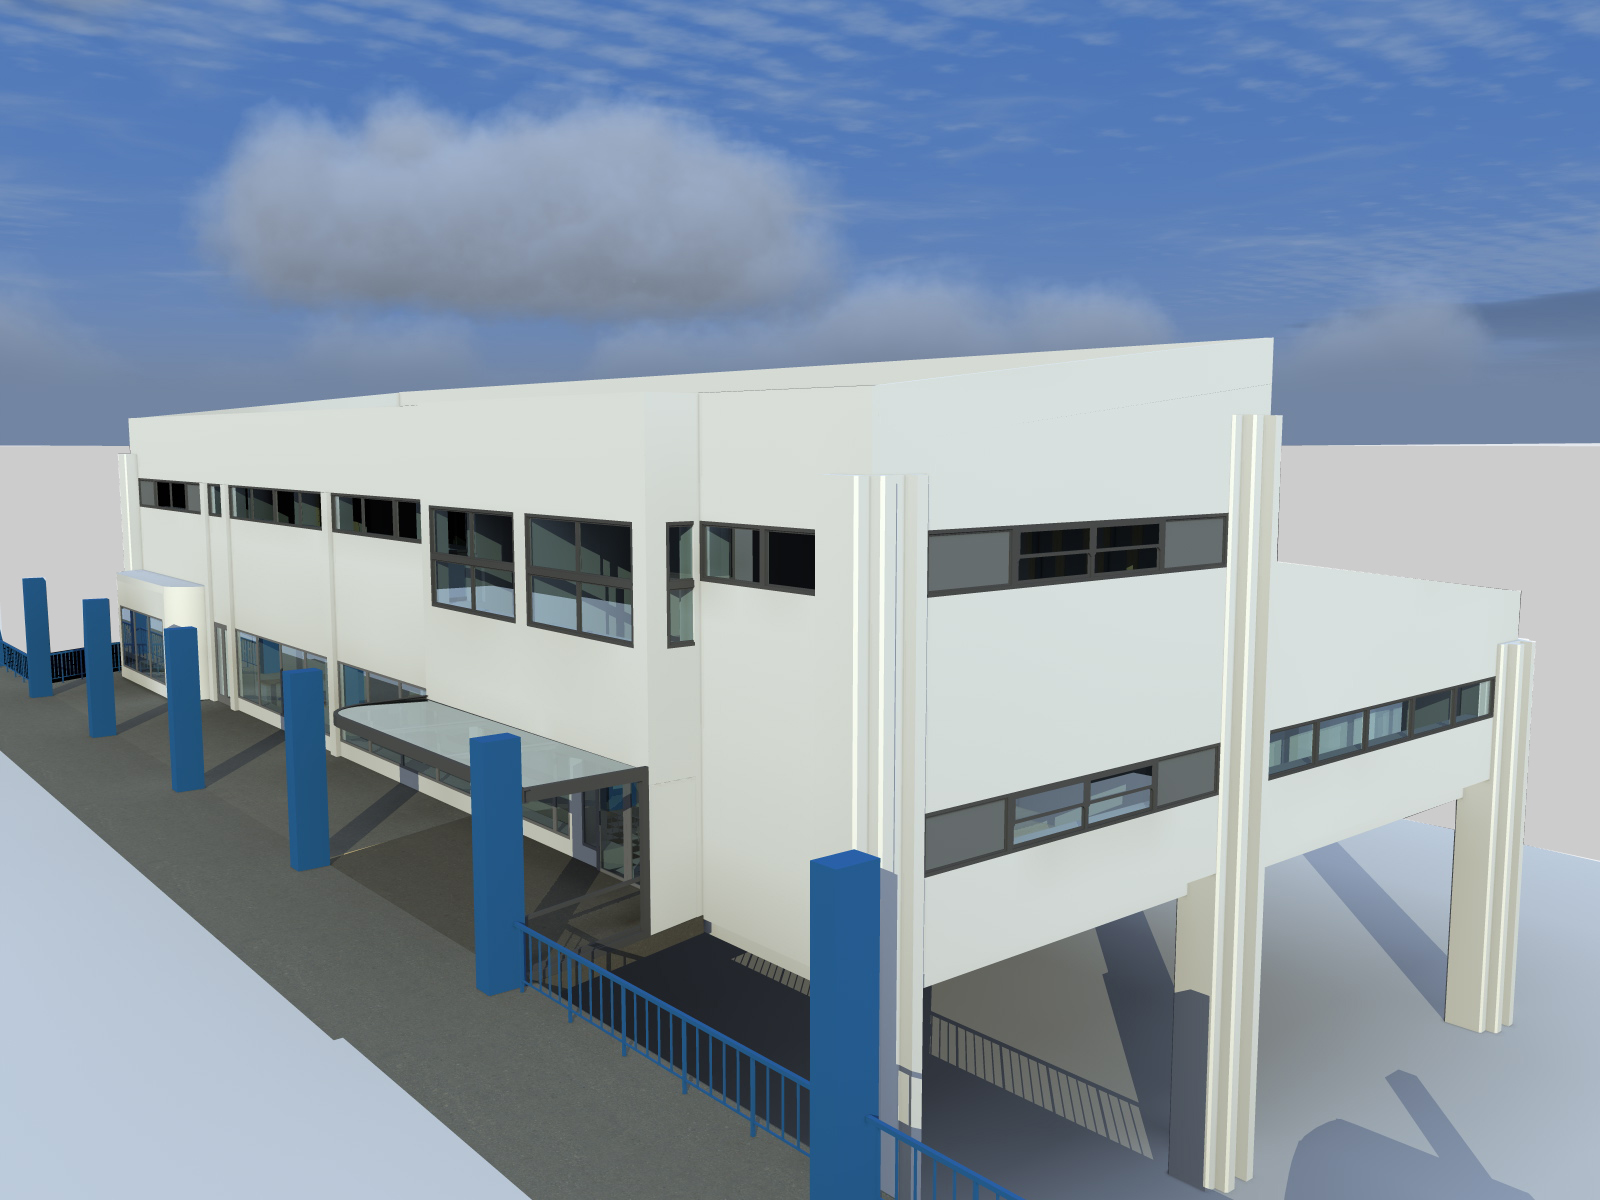
\includegraphics[width=.8\linewidth]{./intro/External.jpg}
  \caption{A render of the proposed changes to the whole exterior (facing onto the Sherfield Walkway}
  \label{fig:sub2}
\end{subfigure}
\end{figure}

Our project comes in 3 parts. The first is to develop playout software which will display content on these large panels, making use of the panels either as several discrete screens, or grouping panels to form large continuous surfaces. The second is to develop a scheduling component, allowing administrators to select and schedule the content shown on these panels. The third is to create an online 'store' where content to be shown on the panels can be viewed, submitted and moderated.

\subsection{Motivation}
The \textbf{Imperial Data Science Institute} \textit{"conducts research on the foundations of data science. Its mission is to foster the development of advanced theory, technology and systems that contribute to the state-of-the-art in data science and big data, notably by funding data-driven research projects and by organizing seminars. The Institute empowers Imperial College and its partners to collaborate in the pursuit of world-class data-driven innovation."}\footnote{http://www3.imperial.ac.uk/data-science}

Despite the exciting world leading innovation happening inside the William Penney Building, its bland looking exterior does not allow passers-by to experience any of the work happening inside. The building is situated on the Sherfield Walkway, one of the busiest parts of the South Kensington campus, due to its centrality in the campus, and also its proximity to the main eating facilities of the campus (the Junior and Senior Common Rooms) and several faculty buildings (Sherfield Building, Huxley Building, ACE Extension). 

Furthermore, the work of the Data Science Institute is unique in that it is very easy to display and present the results of research, in a way that passers-by, regardless of their own areas of studies, can understand, in the form of data visualisations. Many such visualisations already exist and the new projection panels, combined with the large daily footfall, provide a perfect way to increase awareness of the Data Science Institute on campus, and to showcase its latest world-leading research.

We decided to take on this project as we found the scope of the project exciting, the opportunity to revisit and perfect our skills in areas previously explored (such as creating a web application), the opportunity to make use of our more JMC mathematical orientated knowledge (the algorithms used for scheduling) and finally the opportunity to explore new areas of software engineering we hadn't yet experienced in our studies (a GUI application with a large focus on aesthetics and reliability). Furthermore, the project lent itself very well to be divided into 3 discrete parts (the playback software, scheduling, and visualisation catalogue) and so we felt it would be easy to delegate work between the 6 group members, even splitting into smaller subgroups, each working on a different part.

Finally, we were excited to be able to work on something that we may see and come into contact with everyday - \textit{a rare opportunity}.

\subsection{Objectives} \label{sec:intro_objectives}

From the initial project specification, and discussion with our supervisor(s), we started to extract features/objectives we wanted to achieve. We then added these to our Kanban Board (see section \ref{sec:projman_devprocess}) so that throughout development, we had these high-level goals in mind. 

These however did not remain completely static and would change/be added to, based on subsequent discussions with our supervisor(s), as we 'pivoted' towards the best solution.

\begin{figure}[h]
  \centering
    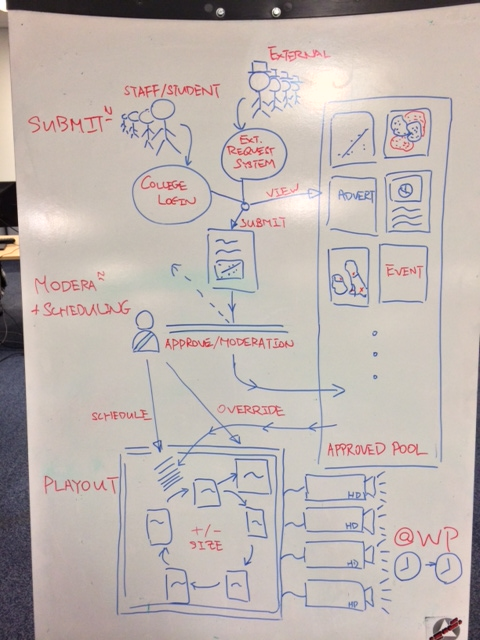
\includegraphics[width = 0.55\textwidth, trim = 0 0 0 1cm, clip]{./intro/userreq.jpg}
  \caption{Initial project specification in a diagram}
  \label{fig:intro_userreq}
\end{figure}

\subsubsection{Primary Objectives} \label{sec:primary_objectives}
\begin{itemize}
\item Users can view visualisations through a web interface
\item Users can submit content to be considered for played back
\item Administrators can moderate submitted content
\item Administrators can schedule content to be played back
\item Content should be served for playback by an intelligent algorithm
\item Scheduling component should be secure from outside attacks
\item Playback system should be robust
\end{itemize}

\subsubsection{Secondary Objectives} \label{sec:secondary_objectives}
(Derived from primary objectives and subsequent discussions)

\begin{itemize}
\item Scheduling should be flexible, but require as little input as possible
\item There should be some guarantee for the amount of time a content item is shown, given its priority
\item Playback system should be aesthetically smooth and not reveal any implementation through its appearance
\item Playback system should not be tied to any specific screen configuration or platform and should intelligently use the displays at its disposal
\item Content can be played back over multiple screens
\item System should rely on Imperial credentials for authentication, by should allow external users to request access
\item Users should be able to 'like' content items and comment on them
\item Allow submitting of both advertisements and visualisations
\item Allow submitting of different formats - images, static web content and videos
\end{itemize}

\subsection{Stakeholders}

Shortly after receiving the project specifications, we identified the stakeholders in our project, their relative importance, and their requirements.

\subsubsection{Administrators}
These are members of staff inside the Data Science Institute who would moderate submitted content, and decide which content items should be scheduled for playback. They require both the moderation and scheduling processes to be as easy as possible, and suited to them, as they are processes which will be repeated very often.

As these users will be using the system most, and the components they interact with are not precisely defined in the specification, their opinion throughout the development process is very important.

\textbf{Requirements}
\begin{itemize}
\item Approve or reject submitted content
\item Choose content to be selected for playback, along with relative priorities and times in which to be shown
\end{itemize}

\subsubsection{Users of visualisation catalogue}

These are users of the web application component of our system. They should be able to view those visualisations which have been approved, and find out more about a certain visualisation and 'like' and comment on a visualisation. This should be done via a modern looking interface (to reflect the cutting edge Data Science Institute) and they should be able to do so on any device of their choosing (i.e. mobile, tablet or through a traditional desktop interface).

Furthermore they should be able to submit content of their own, which after moderation, may be selected for playback. This should be easy to do, supporting a wide variety of formats, and should be done through a slick interface which the user should be confident will get their submission seen.

\textbf{Requirements}
\begin{itemize}
\item View moderated content and interact in a visual and intuitive way
\item 'Like' and comment on content items
\item Submit content to be selected for playback
\end{itemize}

\subsubsection{Users of playback software (passers-by)}

These are students, members of staff and visitors who may pass by or enter the Data Science Institute and see the content projected onto the visualisation panels. They interact with the system in a fairly distant way, and their interaction is fairly well defined - they view the projected content.

Whilst they don't need a large amount of input through the development process, we did identify that how the interact should be aesthetically smooth. They should see content projected correctly, with seamless transitions between content items, and should never have any implementation revealed to them (i.e. an error causing the underlying system to be revealed).

\textbf{Requirements}
\begin{itemize}
\item View projected content
\item 'Like' or vote for interesting visualisations
\item See an ever-changing screen
\end{itemize}


\subsection{Achievements}
We have experimented successfully with new technologies such as AngularJS and Python using the GTk 
library. Most of our previous applications have not contained a GUI, so implementing the playout
system has been a substantial achievement. Also, as it was a requirement for the playout software 
to be cross platform, we had to change our way of thinking when implementing. We had to ask ourselves;
``How would we implement this feature?'' and ``Will this work on Linux and Windows systems?''. This style
of development will help us for future projects.

Away from the technical side of development, we have achieved a good example of an ``Agile'' development
process encorporating multiple features of different development styles, according to our preference. 
We can measure this by looking at our Trello board and meeting notes, and comparing our work to 
previous project cycles. As a group we all stated that we enjoyed working on this project and would 
definitely use the ``Agile'' methodology in future. 

The project has also allowed us to learn how to manage time effectively, especially when juggling 
other academic commitments like lectures and exams. 


\newpage
\section{Project Management}

\subsection{Task Estimation \& Planning}

\subsubsection{Practical Constraints}
The group is acutely aware that with Computing examinations being held at the
end of term, we could only practically carry out development work until the
first week of December. Furthermore, commitments in other courses mean that 
each team member is only able to devote around 16-20 hours per week to
the project. As a group, we have allowed some leeway for each task in case we run into technical errors. If this is the case, we will communicate between the group and come up with a solution if necessary.

In light of these constraints, we have decided to commit to the following:
\begin{enumerate}
  \item \textbf{To maintain a one-week iteration}: this allows the development team to
        obtain maximum possible feedback from our supervisor, who act as our client.
  \item \textbf{To strictly adhere to the original project scope}: while we believe the
        current scope is manageable, we would reject time-consuming items which
        are out of scope before a minimal working system, as mentioned in section ??, is implemented.
\end{enumerate}

\subsubsection{Release \& Iteration Plans}

\begin{figure}[h]
  \centering
    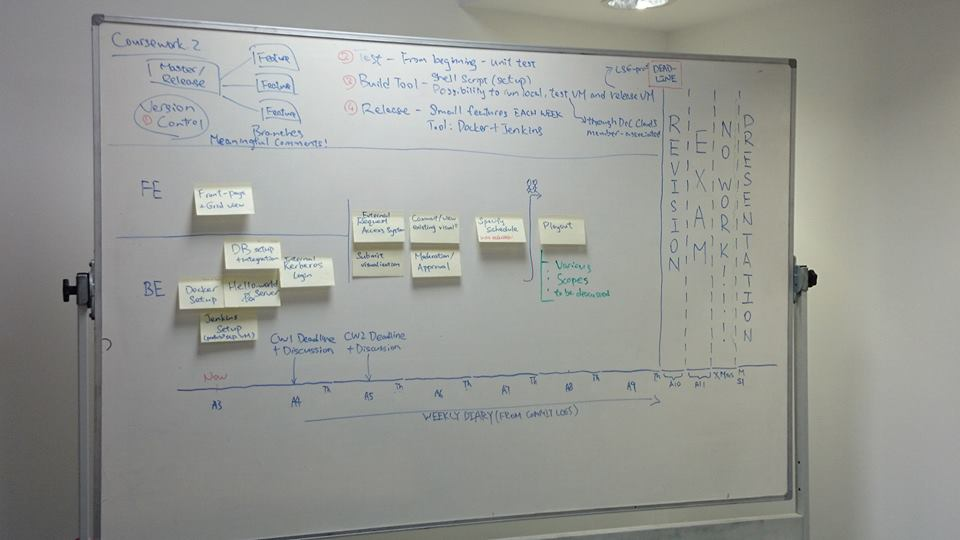
\includegraphics[width = 0.99\textwidth]{./projman/timeline.jpg}
  \caption{Project plan with timeline}
  \label{fig:projman_timeline}
\end{figure}


Taking account of the current project scope, the resultant plan and timeline shown in figure 
\ref{fig:projman_timeline} is a
combination of the plan for next iteration and the release plan, further elaborated in tables 
\ref{tab:projman_rplan} and \ref{tab:projman_iplan}. Each post-it note either represents a 
concrete task to be completed during the next iteration (towards the left), or
high level themes to be implemented (towards the right). Each line segment at
the bottom represents an iteration ending on Thursday, when the development
team will meet with the client.

\begin{table}[h]
  \begin{center}
  \begin{tabular}{c | c | c}
     \textbf{Academic Week (ending date)} & \textbf{Iteration/Sprint} & \textbf{Feature to Release} \\ \hline
     3 \& 4 (30 Oct) & 1 & Infrastructure setup \\
      & & Internal login \\
     5 (6 Nov) & 2 & Access request for externals \\
      & & Visualisation submission \\
     6 (13 Nov) & 3 & Comment/view existing visualisation \\
      & & Admin moderation/ approval \\
     7 (20 Nov) & 4 & Scheduling \\
     8 \& 9 (4 Dec) & 5 \& 6 & Playout \\
  \end{tabular}
  \end{center}
  \caption{Release plan}
  \label{tab:projman_rplan}
\end{table}

\begin{table}[h]
  \begin{tabular}{c | c | c | c }
    \textbf{Iteration} & 1 & 2 & 3 \\ \hline
   \textbf{Tasks} & Front-page \& Grid view & Individual vis$^\textrm{n}$ page template & View/controller hookup\\
      & Docker setup & Configure uploading library & (existing visualisations)\\
      & Hello-world server & Models \& RESTful APIs& Moderation (controller actions)\\
      & Jenkins setup & (for users and visualisations)& Default vis$^\textrm{n}$ seeding\\
      & Kerberos login& Vis$^\textrm{n}$ BG colour extraction & Model extension (comments)\\
      & ... & ... & ...
  \end{tabular}
  \caption{Tasks to be completed for each iteration (partial)}
  \label{tab:projman_iplan}
\end{table}


Estimates on time required for the tasks were based on their relative size and
time taken for us to complete similar ones in the past. For example, some of us
have implemented a College (Kerberos) Login System well within a week, thus if
it is a size M, we can infer that the team (now double the size) is capable in 
fitting two size M tasks within an iteration. For larger system modules, we
assign a longer period specifically for that task: we expect the scheduling
system (size L) and the entire playout system (size XL) would take us one and
two iteration(s) respectively.


\subsection{Group Organisation} \label{sec:projman_group}

\subsubsection{Team Formation}
After we established the requirements of the project, each group member stated
which part of the project they would like to work on. We found that there was a
good split of two people (Andrew \& Emma) that wanted to work on the frontend,
two (Thomas \& Timothy) on the backend server code, and two (Bryan \& Jia Guang)
focusing on database and scheduling.

Although this is a good split to initiate work, we realised that the frontend 
aspect of the project may require more work approaching later iterations.
In addition, we expect that the server code and database should be fully 
implemented within the first four iterations, only requiring minor fixes thereafter.

Therefore, we decided that two people from the backend would move on to creating
the playout software on the dedicated computers; one person would help with the
frontend and the remaining person would apply small fixes and refactors to the
existing server/database code.

\subsubsection{Team Coordination}
% TODO: Chatley: Think about how to synchronise FE and BE work, what if one gets ahead/behind?
TODO

After forming the sub teams, we decided that Bryan and Andrew would be the two respective team 
leaders. This way, they could delegate tasks to specific members at specific times, and give 
deadlines for particular features - formalised via our Trello board.

We also coordinated our work by communicating on Facebook chat. Here we could ask how a particular 
feature was coming along and also organise pair programming in labs. This was particularly useful as 
the whole group could see development progress at the same time. Also, the chat allowed us to use our 
time effectively - if a member needed a particular feature before he/she could start work, then they
could implement a different feature in the mean time. 

Towards the end of the project, we used the issue tracker on Gitlab to let the group know of small bugs.
Although these could be assigned to a specific member, we left them open to the group, so an
appropriate team member could address the issue. 

\begin{figure}[h]
  \centering
    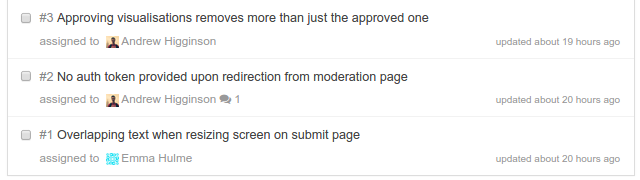
\includegraphics[width = 0.99\textwidth]{./projman/issue_page.png}
  \caption{Small section of the issue tracker on Gitlab}
  \label{fig:projman_issues}
\end{figure}




\subsubsection{Preference on Technologies}
We also asked each group member if there were any specific technologies they 
would like to use, as we realise this project should also be an opportunity to explore new
technologies. After collating these, the member who suggested a technology was then 
tasked with researching more about it, and finding out if it met the requirements of the project.
The member will also be responsible to implement the features with the technology should it be
deemed fit.



\subsection{Development Methods} \label{sec:projman_devprocess}
The team has agreed to adopt a mixture of agile development methodologies to
ensure our practical need and assist the group's working flow.

\subsubsection{General Project Management}

For project management, we generally follow the Scrum method, adopting the
following characteristics:
\begin{itemize}
  \item \textbf{Roles}: We see Dr. David Birch, our supervisor, as the \textit{Product Owner}
        who provide ideas and feedback for the development. At the same time,
        the team have agreed that Andrew should assume the role of
        \textit{Scrum Masters} to facilitate work.
  \item \textbf{Ceremonies}: Upon the initial meeting, we have established a
        meeting with David each Thursday to review our previous sprint 
        and plan our next sprint. We are to hold a development team
        meeting every Monday (figure \ref{fig:projman_scrum}) to update each other 
        on our progress and review work done in past sprints.
  \item \textbf{Artefacts}: We keep our product backlog and iteration backlog on
        Trello as part of our project tracking mechanism (more details
        available in section \ref{sec:projman_tracking}).
\end{itemize}


\begin{figure}[ht]
  \centering
    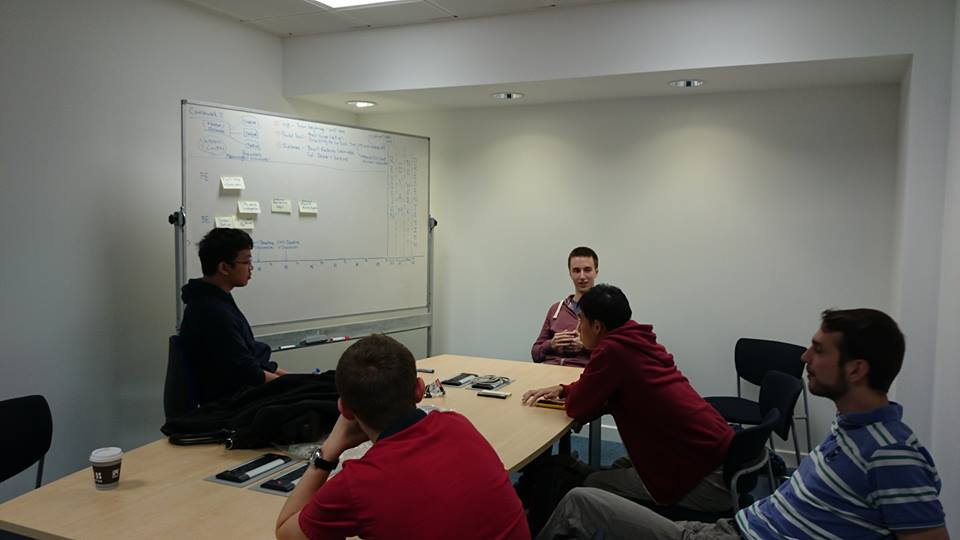
\includegraphics[width = 0.99\textwidth, trim= 0 0 0 3cm, clip]{./projman/scrum.jpg}
  \caption{Half-weekly ``scrum'' (development team meeting).}
  \label{fig:projman_scrum}
\end{figure}

\subsubsection{Technical Practices}

We also integrate a few technical practices inspired by Extreme Programming:
\begin{itemize}
  \item \textbf{Pair Programming}: As mentioned in section \ref{sec:projman_group}, we sorted
        ourselves into three pairs, focusing on frontend (FE), backend (BE) and database (DB) work.
        Such a practice allows continuous development on all divisions without
        being affected by instances in which a member is required to temporarily shift his or her
        focus from the project to other coursework/tests. All members are open to team
        with different members for different tasks, though it turned out members have similar
        preference and usually end up in the same pairs for different tasks.
  \item \textbf{Test-driven Development}: During development, we always write unit and system tests prior to conducting the actual implementation. This ensures individual features are working as expected before we move on to the next feature.

\end{itemize} 

\subsubsection{Project Tracking} \label{sec:projman_tracking}

Finally, to keep track on the group's progress, we use an electronic task
board on Trello (see figure \ref{fig:trello}). Here we can assign ourselves (and others) specific tasks and a general due date. Trello allows us to see what the other members of the group are doing and when a feature is expected to be completed. We can also easily add photos and checklists to see how the project is forming. We decided to use Trello as a physical story-board is not feasible. As well as Trello, we were constantly communicating personally in labs, online via messaging services (mainly Facebook Messenger), and regular stand-ups in a meeting room.

We chose to incorporate this into our way of working, as one of the team members, Andrew, had been involved in projects using Trello, and found it very useful to visualise the work being done on a project.

\begin{figure}[ht]
  \centering
    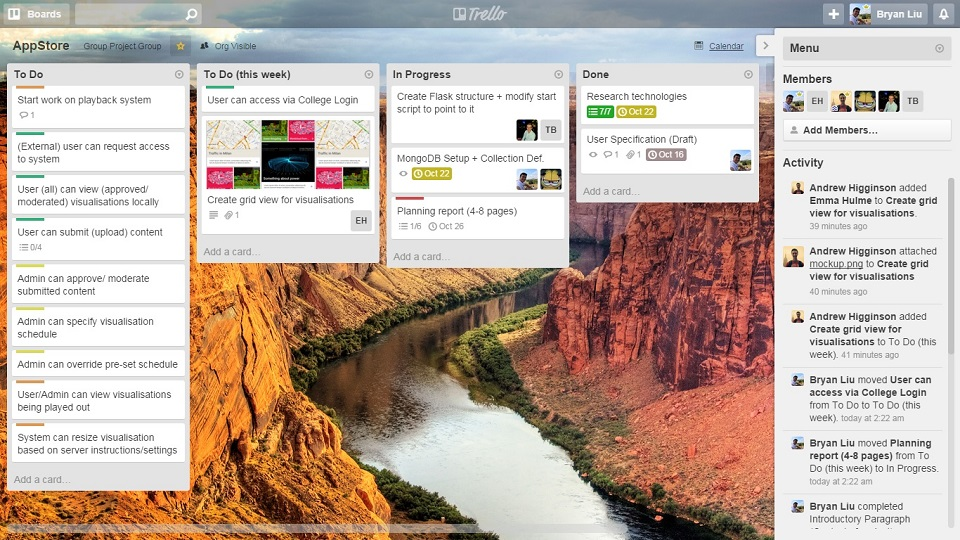
\includegraphics[width = 0.99\textwidth]{./projman/trello.jpg}
  \caption{Using Trello to keep track of progress.}
  \label{fig:trello}
\end{figure}

\subsection{Development Tools}
We have also employed a variety of tools in parallel of our technologies used
in main implementation, illustrated in figure \ref{fig:projman_devtools}, to
enhance our performance.

\begin{figure}[ht]
  \centering
    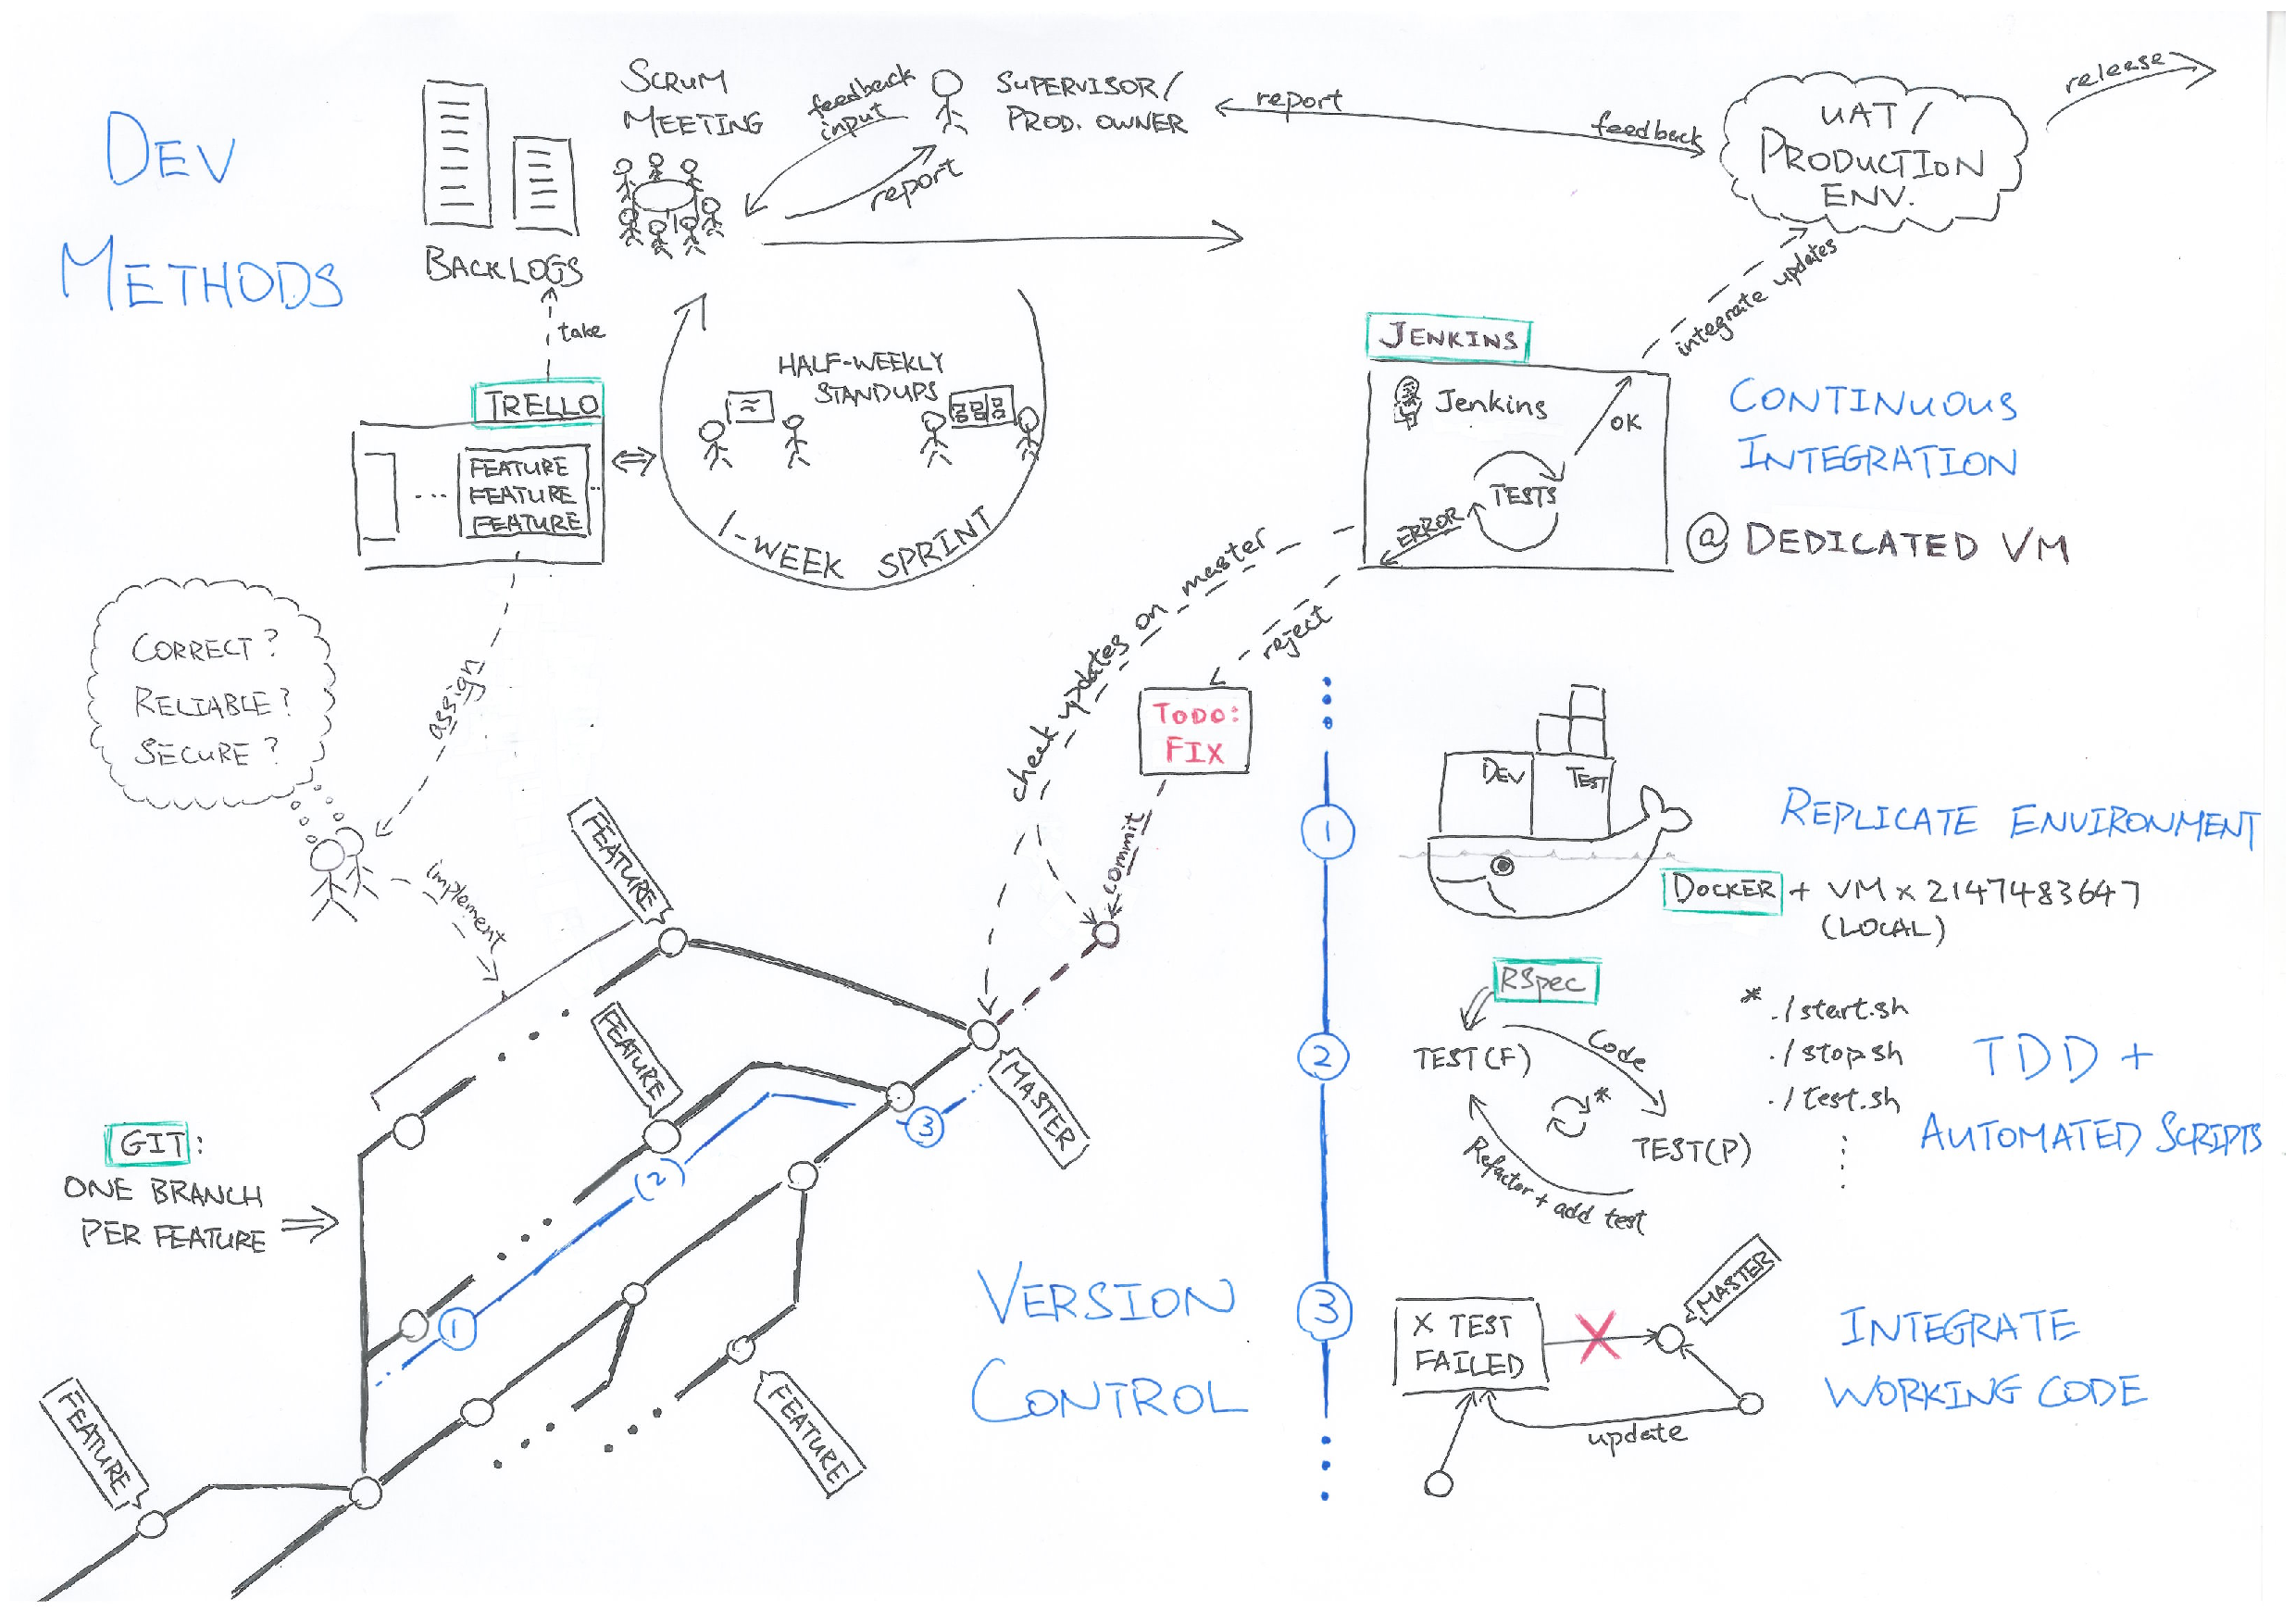
\includegraphics[width = 0.99\textwidth]{./projman/devtools.pdf}
  \caption{Development methods and tools utilised in project.}
  \label{fig:projman_devtools}
\end{figure}

\subsubsection{Unified Development Envorinment} \label{sec:projman_devenv}
%Docker to reproduce dev environment
%Work on own vms in cloudstack within docker container
% Good for testing features away from master

% VM
% Docker

In a group project last year, the backend team had to rely on frontend not in a broken state to ensure a 
particular feature was working. Utilising the newly available CloudStack from the department,
we are able to create a number of virtual machines (VMs) for each feature while it is in development,
and have multiple copies of the web server running from each VM respectively.

While the VM comes nearly for free, they might come with slightly different specification,
which might cause discrepancies further into development. After a lecture on deployment techniques, the group decided to use Docker. Docker allows us to quickly set up standardised VMs (containers), installing any dependencies we need automatically. Although it may be a steep learning curve at the start of our project, it proves that Docker saved us a lot of time, 
for instance ensuring all supporting libraries exist in local VM.

To further speed up development process, we have also written a number of automated scripts
to build Docker images (templace for a container VM), as well as starting and stopping the
webserver when called.

\subsubsection{Version Control}
The team has decided to continue using Git as our version control system, as all of us have had
at least two years of relevant experience from previous projects and laboratory work. Furthermore,
Git is supported by multiple OS platforms with minimal configuration (e.g. end-of-line CRLF/ LF conversions),
allowing one to continue their work should a linux machine, for example, is not available.

As usual, all of our code (including the scripts mentioned in \ref{sec:projman_devenv}) 
are stored in a group git repository on the department's GitLab server. Instead of naming branches under team members'
name and working under it individually for the entire project span, we have decided to use branches with a short lifetime.
Each minor feature is implemented on it's own branch, and the master branch is only used for merging in features for release
after being tested locally on its own branch and associated local VM (see section \ref{sec:projman_tdd}).
Such practice makes it easier for different team members, under pair programming, to work on the same feature.
It also makes it easier for the team to backtrack and locate the bug should any problem arise by checking a small number of commits on that particular branch.

Moreover, with meaningful yet concise commit messages, we can effectively
communicate with each other what we have done along with updating our task-board
on Trello and sending messages on Facebook Messenger.


\subsubsection{Test-driven Development} \label{sec:projman_tdd}
With Ruby on Rails being our choice of implementation language (refer to section \ref{sec:impl_RoR}),
RSpec is inevitably the obvious choice for testing server codes.
While it is nicely integrated with Ruby on Rails, with test templates automatically
generated along with new code segments (models and controllers);
tests written with RSpec is highly human-readable and thus
easing the difficulty in maintainence as the tests themselves are already
decent documentation of our implementation.

We also have an automated script to run all written tests in a seperate
environment (Docker container) without affecting the webserver, minimising
the disruption to the server's normal operation during development.


% RSpec - Nice integration with RoR
% Failed test - imp - passed test - (refactor) cycle
% Another automated script to run all test in seperate Docker container

\subsubsection{Continuous Integration \& Build Promotion}
% Jenkins installed on a release vm
% Tests code every time we push to master by pulling it
% Tells us quickly if something is wrong

While it is cumbersome to manually stop, test and restart the server
everytime we implement a feature or provide a fix, we have
included a Jenkins instance in our release virtual machine to automate
the code integration and deployment process, allowing us to focus on
development.

Our Jenkins instance is equipped with a GitLab hook: upon any team member's
commit towards the master branch of the project git repository, the hook would
automatically execute a short script which pulls the updates, runs the tests
on the updated code and integrates the updates. If something went wrong,
Jenkins would notify us immediately and we could look at the issue and get
it resolved as soon as possible.

This feature also meant that our supervisor, David, could look at the release vm 
for the most up to date version of our web application. 


\newpage
\section{Design and Implementation}

\subsection{Implementation Tools}

\subsubsection{Front-end: }
% TODO Andrew: please add section headings as appropriate
TODO 

FE: 
  angular for one-page smooth application
  google material design guidelines

For the frontend, given the amount of similar web application projects Andrew and Emma had worked on, they decided to explore using AngularJS, as a different way of implementing frontend logic. They have since decided to use it, as it allows interfaces to be programmed declaratively, making it much easier to 'see the behaviour' of the UI from code.


\subsubsection{Back-end: Initial Attempt - Flask (Python) \& MongoDB}

During the inital phases of our project, we decided on which tools/technologies to use based on our personal preference. For the backend, we decided to use Python with Flask. Members of our team had previously used Ruby on Rails and Python with Django, so we decided to use Flask for interest purposes. To make sure Flask was suitable, the backend team spent time researching additional modules that would allow us to implement future features.


% Advantage of MongoDB - fast read, scalable, JS-like (easy FE adaptation)
As Bryan and Jackie were more interested in the database side, they chose to use MongoDB as a NoSQL
solution. Again, this was based on interest. We see MongoDB especially helpful especially in early
development stage when the schema is not well-defined, as MongoDB is flexible with document-oriented,
dynamic schemas. Moreover, we believe MongoDB's ability in supporting fast read and scalability would be
beneficial to the project in long-term. Bryan used time at the beginning of the project to check that 
Flask was compatible with MongoDB and found it is possible with the library \texttt{Flask-PyMongo}.

% Problems - broken kerberos adapter, (changed from flask as we were getting stuck - consulted with David)
After about a week of usage, we found that there had been lots of small problems in development. After 
experimenting with a Kerberos authentication module for Flask, we found that the documentation was 
very poor and some behaviour was erratic. Also, creation and maintenance of the database was taking 
longer than previous web projects. 

As a group, we decided that it would be beneficial to switch technologies to Ruby on Rails, as we had
previous experience and was quicker to set up. We consulted with David in our weekly scrum, who was
happy for us to change. The change would not affect end users of the system, and would still enable us 
to develop in the same environments. 

\subsubsection{Back-end: Finalised Use - Ruby on Rails} \label{sec:impl_RoR}

We used our previous experience in Ruby on Rails to quickly and easily set up the project. We could also
use a wide range of gems for particular features, especially for authentication users with the college
Kerberos servers. Using rails also meant a smooth interaction with the database, which also required 
little setup. In the first few days of development we noticed that we were implementing features much
faster and feeling more confident with the work that lied ahead. 

We decided to use Java to initially write the scheduling algorithm, which would then be translated to 
Ruby. This was because we were more confident with Java, and it's object orientated paradigm would make 
the algorithm easier to implement. We thought (correctly) that this method would be quicker than
implementing the algorithm in Ruby from the outset. Intelligent design and use of comments meant that
the resulting Ruby code would be well structured and efficient.
  

\subsubsection{Playout Software: }
For the playout software, we decided to use Python with the Gtk graphics library. This was partly down
to previous experience with Python but mostly because we needed the software to be cross platform. Hence,
when developing the playout software, we used dual-boot Linux and Windows machines to test after every 
feature was implemented. 

To continuously poll our server, we used timers in python, to make sure the software displays the 
current visualisation. We also wanted to hide any Windows/Linux GUI elements, e.g. scroll bars, so we 
made use of customised ``Web Kits''.


\subsection{AppStore Design}

% Feel free to add more subsubsections!

\subsubsection{Architecture}

\begin{figure}[ht]
  \centering
%    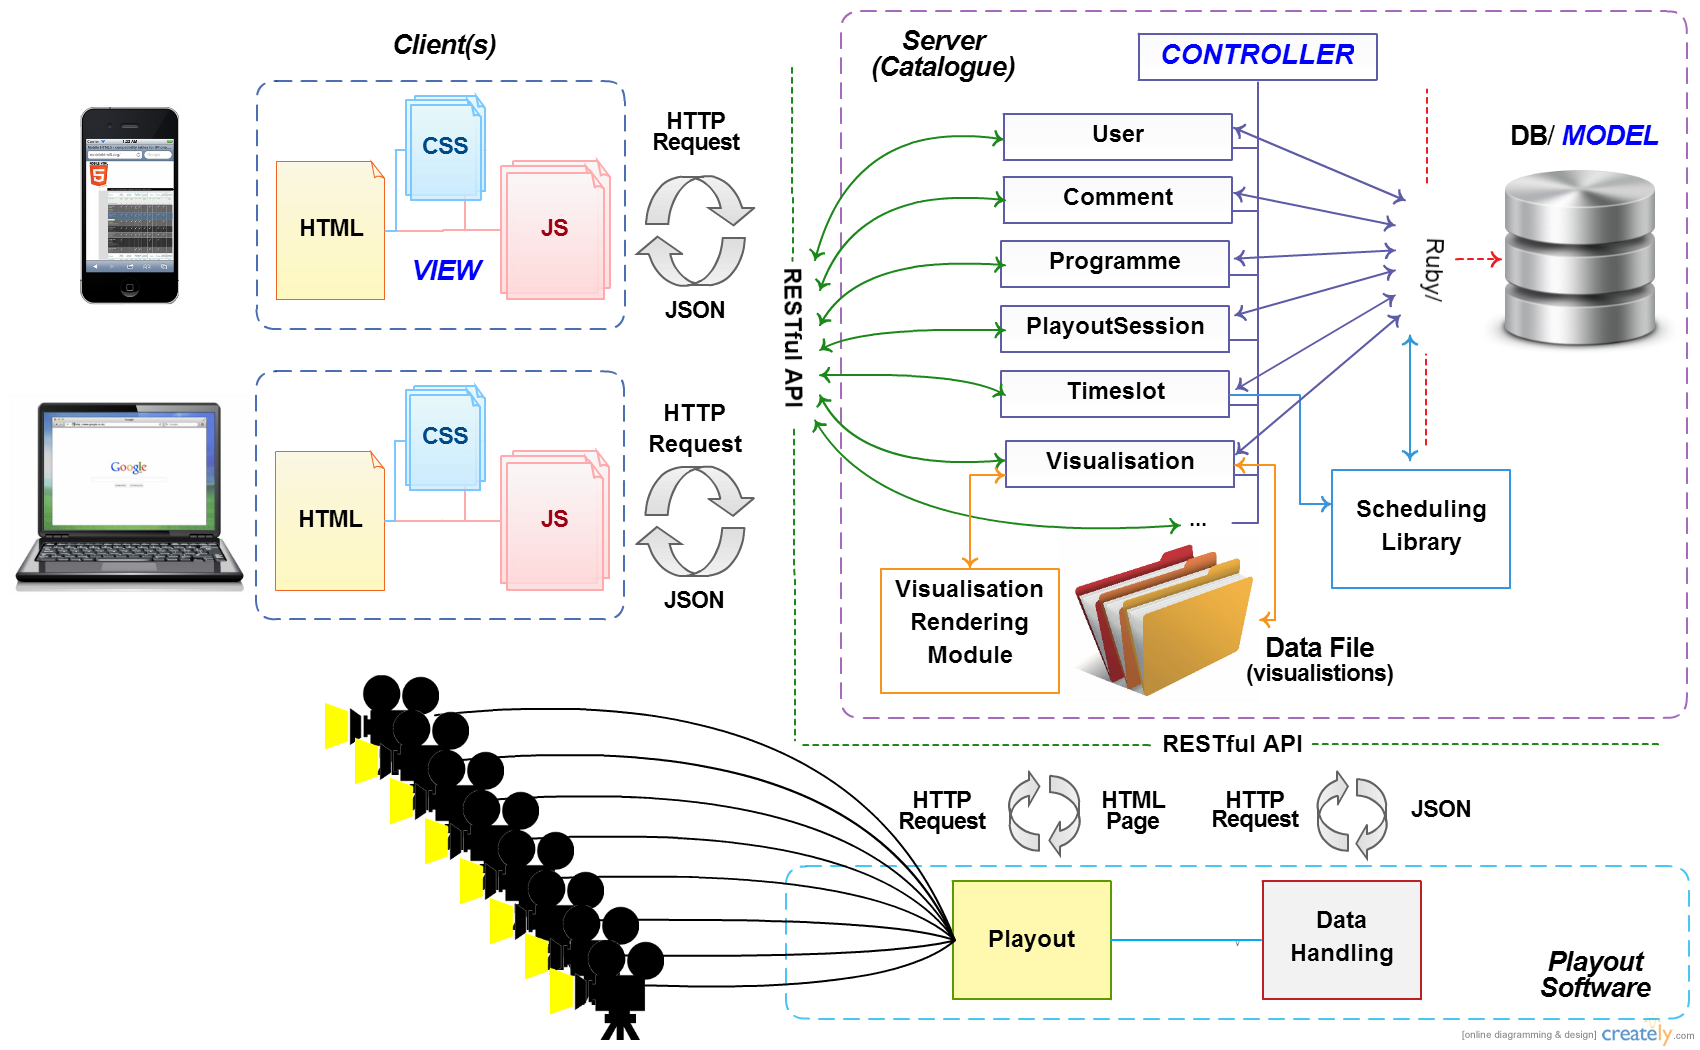
\includegraphics[width = 0.99\textwidth]{./impl/architecture.jpg}
  \caption{System architecture for the AppStore}
  \label{fig:impl_models}
\end{figure}

% Diagram on system architecture, showing RESTful API, HTML gets and playout software gets
% RoR enforces MVC architectural pattern

\subsubsection{Models}

\begin{figure}[ht]
  \centering
%    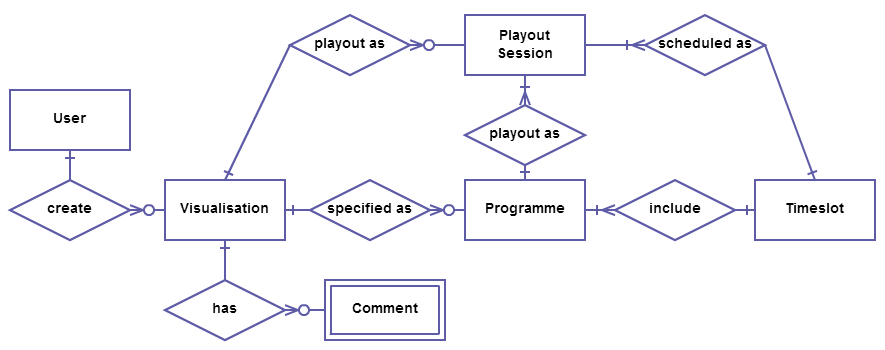
\includegraphics[width = 0.99\textwidth]{./impl/models.jpg}
  \caption{Models of entities and resources in system and their relationship}
  \label{fig:impl_models}
\end{figure}

% Diagram for model relationship
% 1 or 2 paragraphs for each model - what it represents/does, relate to the objectives in section 1

A \textbf{user} ...

A \textbf{visualisation} ...

A \textbf{comment} ...

A \textbf{programme} ...

A \textbf{timeslot} ...

A \textbf{playout session} ...


\subsubsection{Controller Actions}

% Briefly describe controller actions which requires routing, etc. - what it does 

% Andrew: is it worth to write a view section?
% \subsubsection{Views}


\subsubsection{Scheduling Library}

% Jackie: Brief mention of the library and the functions (high-level)
% Tom: Description on middle-man

As the scheduling library was implemented separately from the request controllers,
we needed a middle-man to call the scheduling functions. When a timeslot is edited, i.e. 
visualisations/adverts where added to it, the scheduling function is called from
the controller and the playout session records are created in the database. Any 
subsequent changes to a timeslot clears the sessions that the scheduling algorithm 
has previously created for it, and generates a new schedule. 

\subsubsection{Playout Software}

% TODO: Working mechanism - how it grabs visualisation, rendering, QR...



\subsection{Technical Challenges \& Risks}

% TODO: Any technical challenges encountered and how addressed?
% TODO: Any risks anticipated, and how mitigated
% Please feel free to introduce subsections

\subsubsection{From Java Scheduling to Ruby Scheduling}
% Translation on scheduling from Java to Ruby

\begin{figure}[ht]
  \begin{minipage}{0.49\textwidth}
%    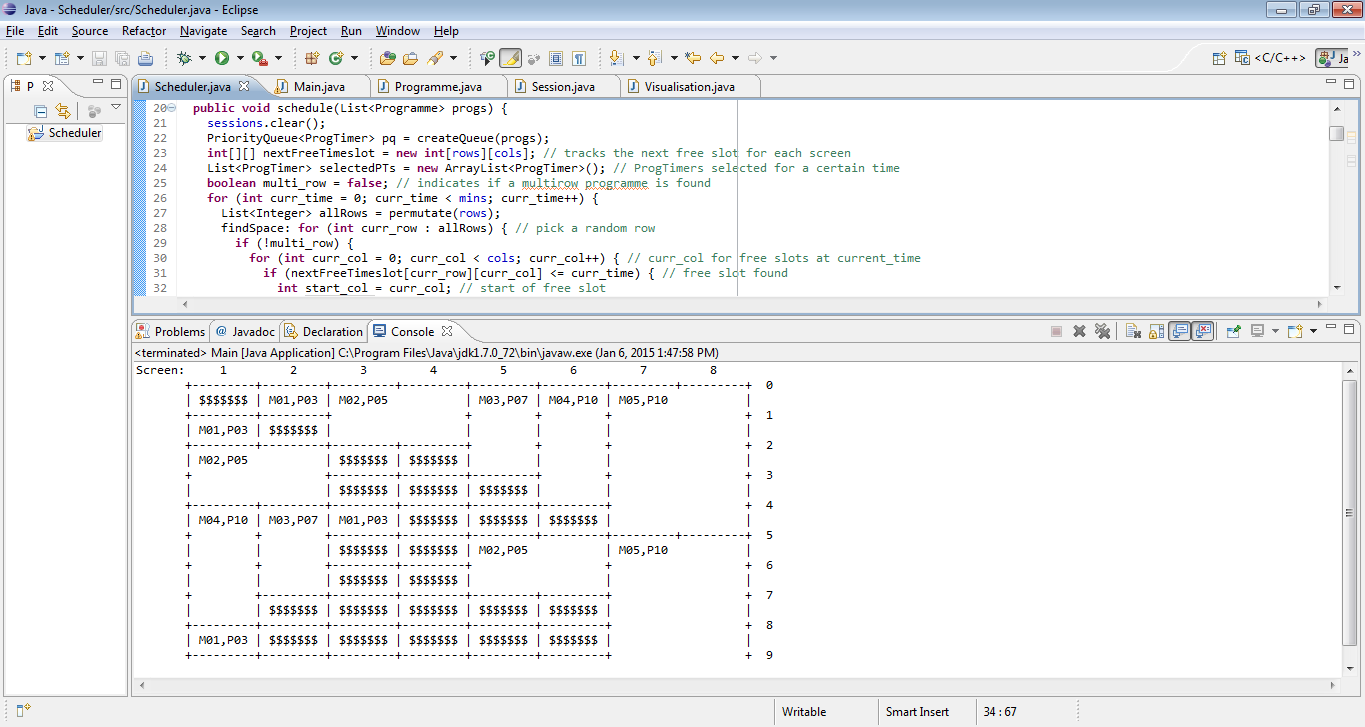
\includegraphics[width = 0.99\textwidth]{./impl/java_scheduling.jpg}
  \end{minipage}
  \begin{minipage}{0.49\textwidth}
%    \includegraphics[width = 0.99\textwidth]{./impl/ruby_scheduling.jpg}
  \end{minipage}
    
  \caption{Implementing scheduling libarary in Java (left) and translation to Ruby (right)}
  \label{fig:impl_translation}
\end{figure}


\subsubsection{Security}



\newpage
\section{Evaluation}

\subsection{Stakeholder Relationships}

\subsubsection{Stakeholders}

The main stakeholder in our project is our supervisor, David. The core of our project is the scheduling component, which he will operate as an administrator, so his opinion of the overall design of the project is critical.

Our second class of stakeholders are those who browse the visualisation catalogue and submit visualisations and advertisements. Their stake is relatively large as without their full engagement and satisfaction, the variety of content being shown will remain small. 

Our last group of stakeholders are those who see the visualisations being played out. While this set of users are still important, their stake is relatively small, in that all they want to see is the content being played out successfully.

\subsubsection{Customer relationship}

Where customer relationships are concerned, we see our most important stakeholder, our supervisor, David, as somewhere between an internal and external customer, whom we hold weekly meetings and exchange emails frequently with but not contact in person daily. During weekly meetings, we explain the features that are in progress/to be done over the next week, so that David is always kept in the loop (Figure \ref{fig:eval_meetingboard}).

We tended to keep discussions fairly high-level, and only discussed implementation details/technologies when asked to do so, or when we felt that it was important to the discussion. We did this to mimic the scenario of David being our client, but also to ensure that discussions were not biased towards any kind of implementation, allowing us to fit our implementation around the best ideas, and not the other way around.

\begin{figure}[ht]
  \begin{minipage}{0.49\textwidth}
    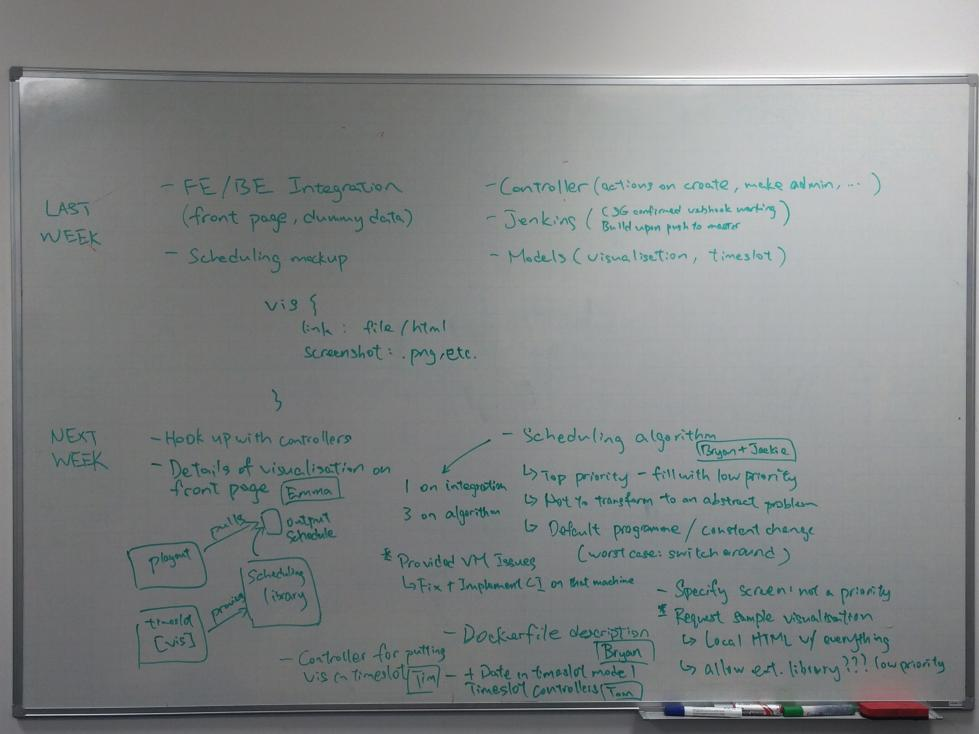
\includegraphics[width = \textwidth, trim = 0 0.4cm 0 1.6cm, clip]{./eval/meeting-board2.jpg}
  \end{minipage}
  \begin{minipage}{0.49\textwidth}
    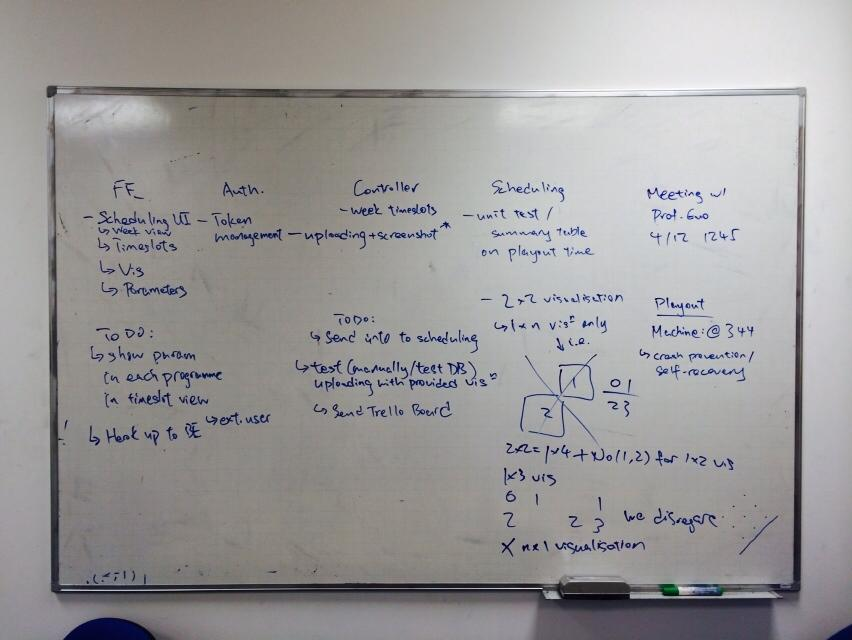
\includegraphics[width = \textwidth, trim = 1.2cm 1.5cm 1.2cm 2.5cm, clip]{./eval/meeting-board.jpg}
  \end{minipage}
  \caption{Meeting notes with group progress and feedback from David (our supervisor) after sprint cycles 2 (left) and 4 (right).}
  \label{fig:eval_meetingboard}
\end{figure}

Furthermore, with the aid of Jenkins, we are able to give the address of our ``release VM'' to David, where he can see the latest working version of the project. From this, David can constantly evaluate and provide feedback on our project features through all stages of development.

\subsubsection{Feedback handling}

Upon receiving feedback from our stakeholders, mainly from our supervisor, we handled them depending on their nature:

\begin{itemize}

  \item Change in minor details of a feature/design: \\
        Usually happening in the prototype stage, they include changing font size/colour and displaying some extra information on a screen. As these changes take only a few hours at most to implement, we took the majority of such suggestions and fitted these XS-items in the next iteration.

  \item Introduction of new, peripheral features: \\
        These include features that are related but not essential for our three main components (submission, moderation/scheduling and playout): Multiple default playout lists, playing videos with linked themes consecutively, buttons to copy and paste previous timeslots, etc. \\
        However, due to time limitations, we chose to integrate only one or two small-sized features into our planned implementation. The rest of the suggested features were put into an ``extra feature" list, which we only considered implementing after basic versions of the main components are completed. This ensures that we can produce a minimal product at the very least before our planned deadline.

  \item Major changes in feature implementation: \\
        As a result of differing assumptions, the feedback necessitates the changing of what we have already implemented. For instance, we were required to change the priority rules in our scheduling algorithm. When this happens, we spend a significant portion of the weekly meeting to clarify the assumptions that our supervisor has made, and try to combine them with our own assumptions and implementations. This feedback has sometimes resulted in some or all of our code being scrapped, but it generates a product which is more useful to our stakeholders.

\end{itemize}

In all cases, we have communicated with the personnel that provided the
feedback with justification on our decisions. For example, we told
our supervisor that we are happy to accede to his request of adding a button which copies previous timeslots as we rate it as a S-sized task which can fit into the planned iteration, but his request for linked videos to be scheduled to be screened consecutively would delay our plans, and thus should be considered only after the entire system is implemented minimally.

\subsection{Product Requirement, Value \& Impact}

In the first week of embarking on our project, we met with our supervisor to highlight the initial components required. At first, these were general
requirements including:

\begin{itemize}

  \item Stakeholder requirements resembling user stories (e.g. a user is allowed to submit scientific visualisations and/or advertisements, as well as to state his/her preference(s) on playout).

  \item System/Interface requirements - what users expect it to be able to do based on the user stories above (e.g. The scheduling system should schedule items to play out in rotation, so that passers-by will not be bored by the ``fixed" playout sessions).

\end{itemize}

In the following weeks, we then clarified and expanded on these requirements as a group. This allowed us to discuss the implementation and technical details of specific features.

\subsubsection{Value Proposition}

We also further clarified our understanding of stakeholders and how our system creates value for them via multiple value proposition canvasses. Figure \ref{fig:valpropcanvas} shows the canvas for the Imperial Data Science Institute, which our supervisor is associated with. It includes a customer profile with a list of jobs, gains and pains, and corresponding products/services, gain creators and pain relievers (value map). Some of the gains/pains of the institute, along with their creators/relievers are as follows:

\begin{itemize}

  \item Gain: Makes the walkway more interesting (by showing visualisations to passers-by)

  \item Pain: Requires a large number of visualisations (relieved by inviting users to submit visualisations)

  \item Gain: Creates income opportunities (by showing adverts)

  \item Pain: Attracts inappropriate submissions from users (relieved through admin moderation)

  % Put the 3rd pair of gain/pain in

\end{itemize}

The canvasses enable us to disregard features that deliver low or no value, and make more reasonable assumptions about our stakeholders. We believe that the latter has resulted in fewer problems for us when we began our product validation, detailed in Section \ref{sec:validation}.

\begin{figure}[ht]
   \begin{center}
      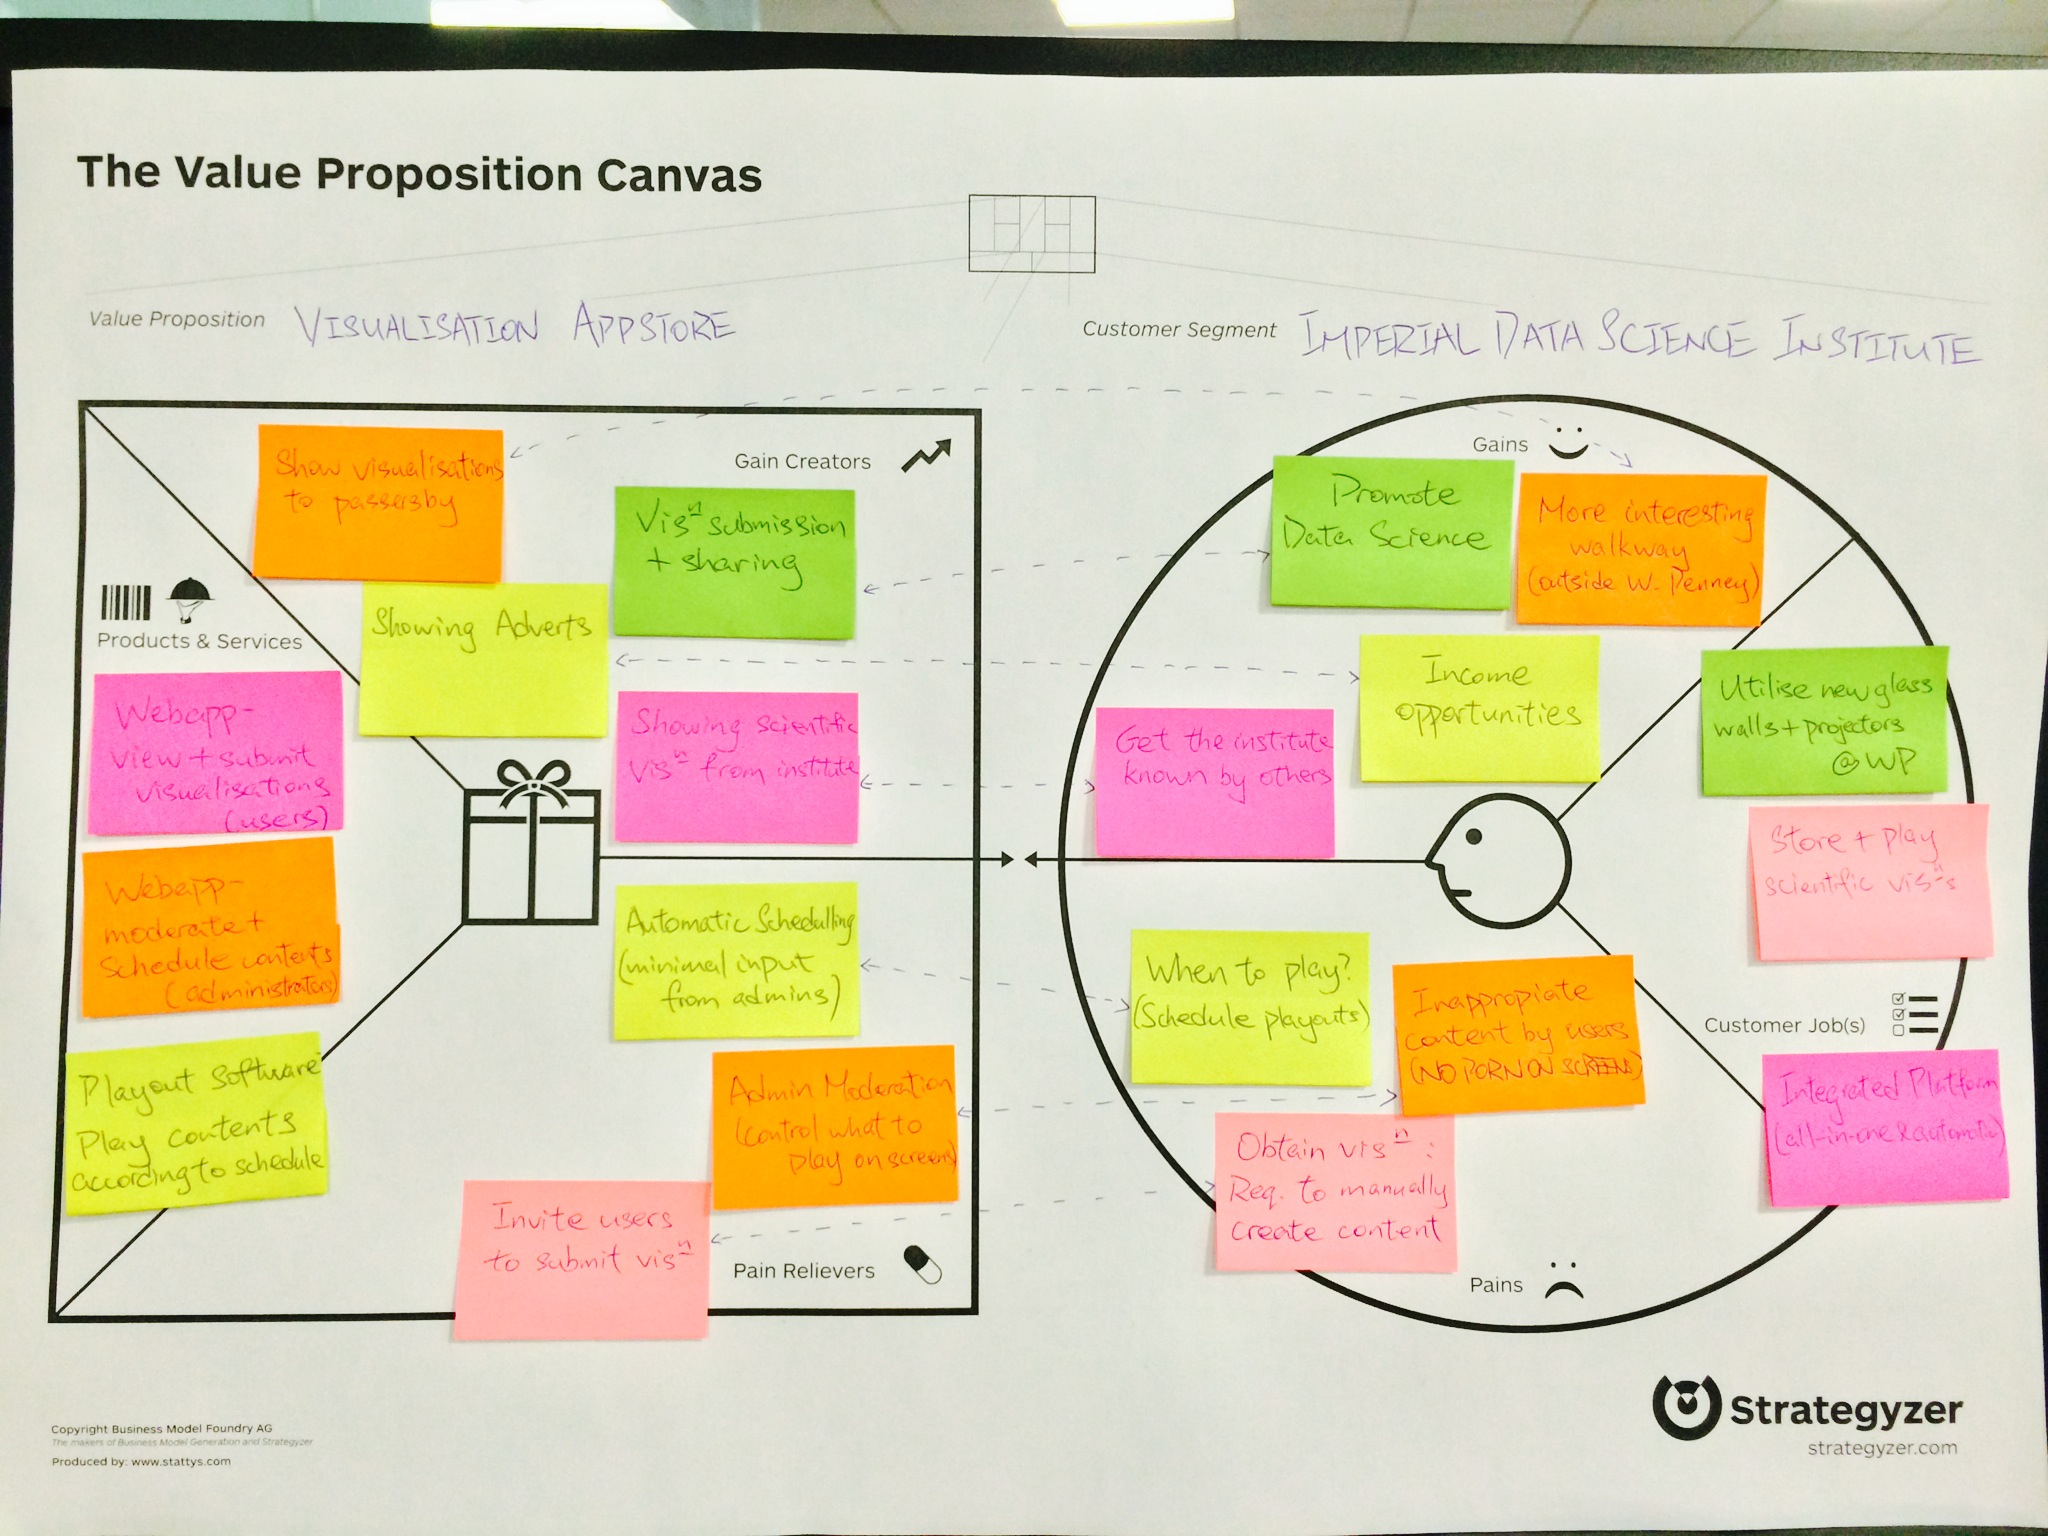
\includegraphics[width = 0.9\textwidth, trim = 1cm 6.5cm 1cm 4.5cm, clip]{./eval/value_prop_canvas.jpg}
   \end{center}
   \caption{Value proposition canvas for our client (Imperial Data Science Institute).}
   \label{fig:eval_valpropcanvas}
\end{figure}

\subsection{Task Management}
During development, we constantly looked at the requirements from all of our stakeholders, which we stored in a shared document. In our weekly scrums, we presented the work that we have done to one another and discussed whether the project is on the right track.

We prioritised tasks on our Trello board using different columns. In addition, we constantly communicated both face-to-face and online, to make sure that group members are implementing assigned tasks at the right times. We also used the Trello board actively to update the rest of the group when tasks have been completed, hence saving us the trouble of constantly asking the rest of the group or looking at code to find out if a feature has already been implemented. When appropriate, group members working on the backend used an internal wiki on Gitlab to provide information about routing, controller actions, and parameters. 

\begin{figure}[ht]
  \begin{minipage}{0.49\textwidth}
    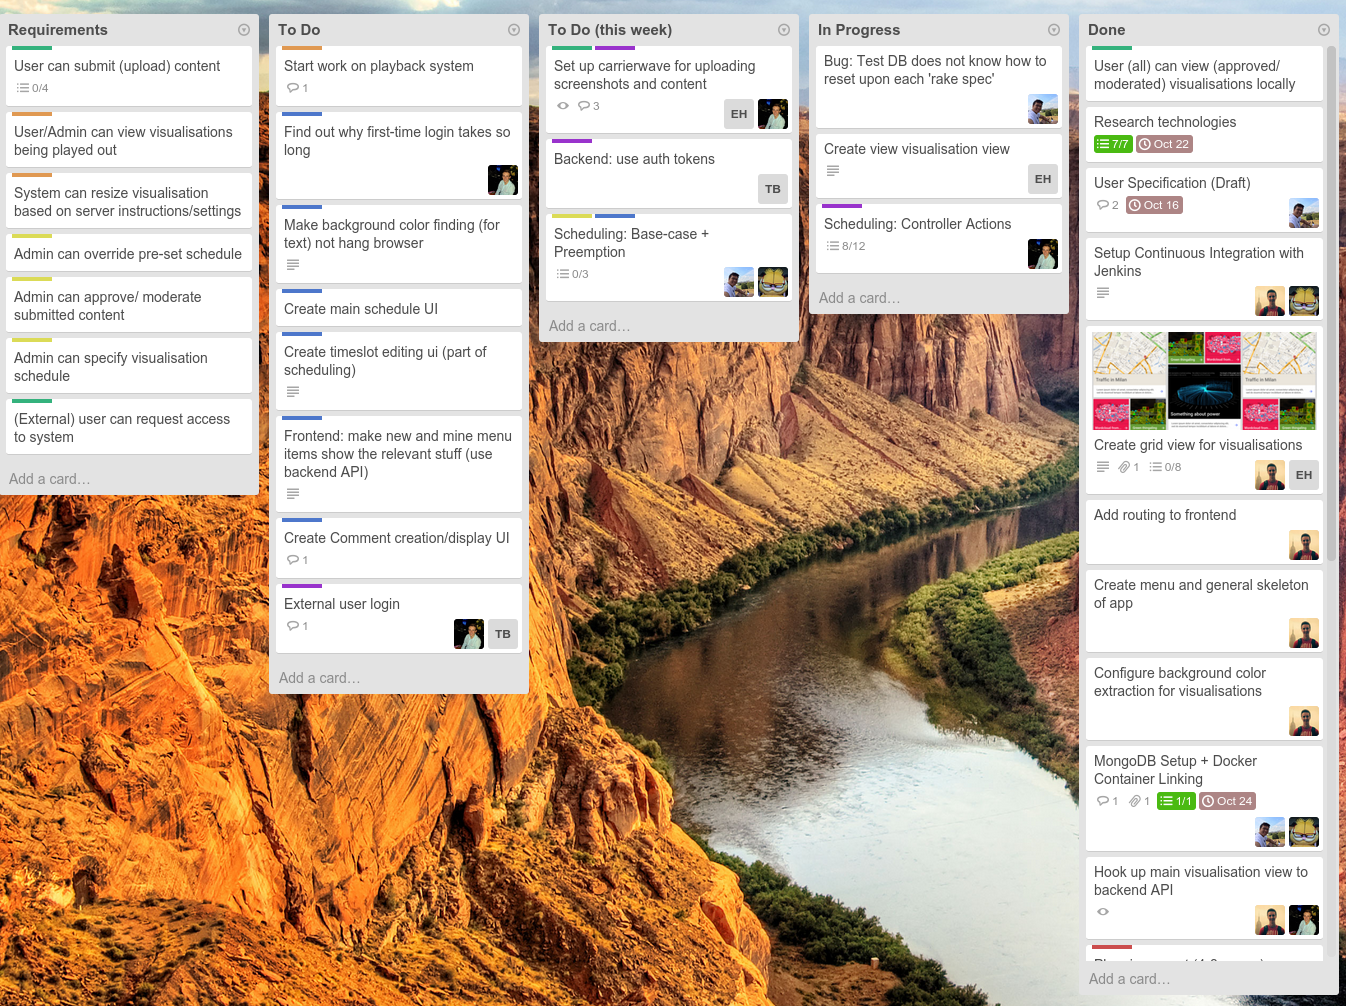
\includegraphics[width = \textwidth]{./eval/trello-columns.png}
  \end{minipage}
  \begin{minipage}{0.49\textwidth}
    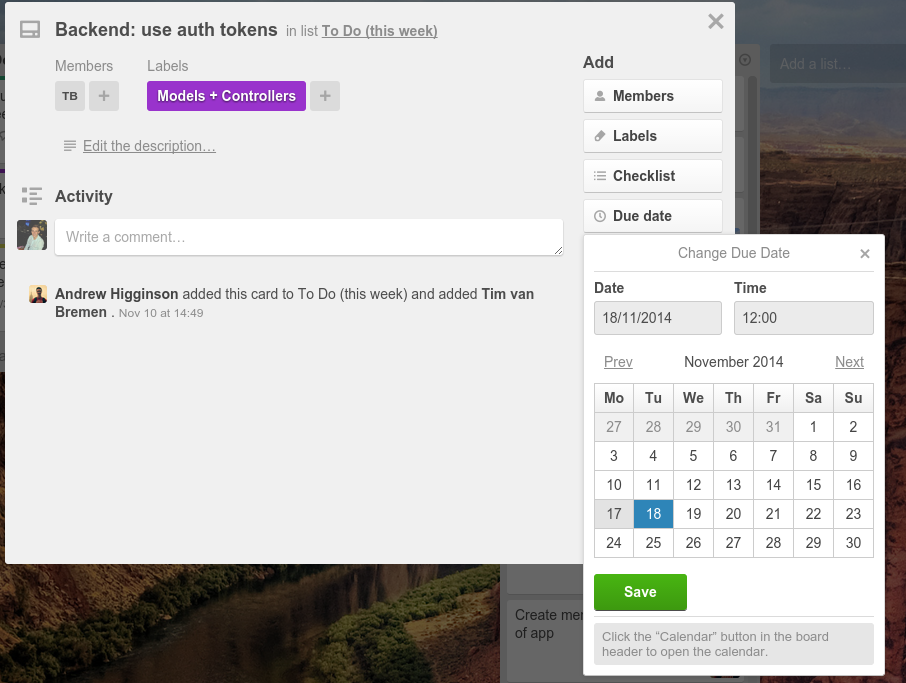
\includegraphics[width = \textwidth]{./eval/trello-due-date.png}
  \end{minipage}
  \caption{Priority columns on our Trello board (left); \\Setting a due date for a particular task (right).}
  \label{fig:eval_trello}
\end{figure}

\subsubsection{Story Splitting}

While some of our project requirements can be completed within a few hours, other features are unlikely to be completed within one iteration. In such cases, we split the features into multiple units and implement them in different iterations based on their priority.

An example can be found in the following user story:
\begin{center}
``\textit{As a user, I want to access the platform via a set of credentials so that I can upload visualisations (user)/perform moderation and scheduling (administrator).}'' \\
\end{center}

We considered this task to be technically challenging. Hence, we split it into the following subtasks:

\begin{itemize}

  \item As an internal user (student/staff at Imperial), I want to access the platform via my college login so that I can upload/moderate and schedule visualisations without the need for an extra set of credentials.

  \item As an external user, I want to access the platform via some kind of access request system, so that I can share my visualisations too.

\end{itemize}

In addition to being reduced in size, splitting the story has also helped us further understand the needs of different groups of users. As such, we decided to implement the former requirement first, as some of our team members have had experience on working with the college login system, hence allowing the requirement to be fulfilled in a shorter time. The latter requirement was then scheduled to be carried out in parallel with the mentioned features.

\subsubsection{Spikes - Experiments with new technologies}

Throughout development, we also devoted a small proportion of time to experiment on technologies involved in later iterations. This allows us to better understand the potential complications that we will face and react accordingly.

While we planned to implement the playout system only in iterations 5 and 6 (the last two iterations), investigation on relevant technologies, including Qt and its adapters, were made from iteration 2. Preliminary research allowed us to confirm that 2 weeks would be a reasonable estimate in system implementation. Furthermore, we believe that the investigation would result in a more gentle learning curve, and reduces the risk for development grinding to a halt as team members will at least have some basic knowledge on Qt, and some code segments will be produced.

However, not all spikes bring good news - investigation on Kerberos login libraries has revealed that the adapter for Flask (with Python) is actually broken, forcing us to scrap the entire implementation. Nonetheless, the spike allowed us to switch our choice of development language early and avoid incurring high costs further into development.

\subsection{Building the right thing - Assumption Validation} \label{sec:eval_validation}

Given the tight deadlines for the entire project, we agreed to collect
user feedback as soon as the project commenced. This ensures that we are building the right product for our stakeholders.

\subsubsection{UI mockups/ prototypes} \label{sec:eval_uimockup}

Before implementing a particular part of our project, we begin with creating mockups (Figure \ref{fig:eval_mockup}). These can be produced in a relatively short time, and allows us to quickly think through the design of our project, without being tied down to any implementation details. After completion, we show the mockups to the main stakeholder in the project i.e. our supervisor, who gives us feedback. For example, he mentioned that it will be a good idea to show the priorities associated with each visualisation in the timeslot views, even if the visualisation is not selected after viewing the mockups.

Once we have settled on a general design, we complete the main implementation of the UI within that week's sprint cycle, but only up to the point where we can see how it will be used. As it is not interacting with the backend at this point, small changes are easily implemented, with the following week's sprint cycle involving ``hooking'' up this UI prototype with our backend.

We also made sure that this prototype is seeded with some dummy/representative data in some way, so that it is clear how each part of the project will operate in practice.

\begin{figure}[ht]
   \begin{center}
      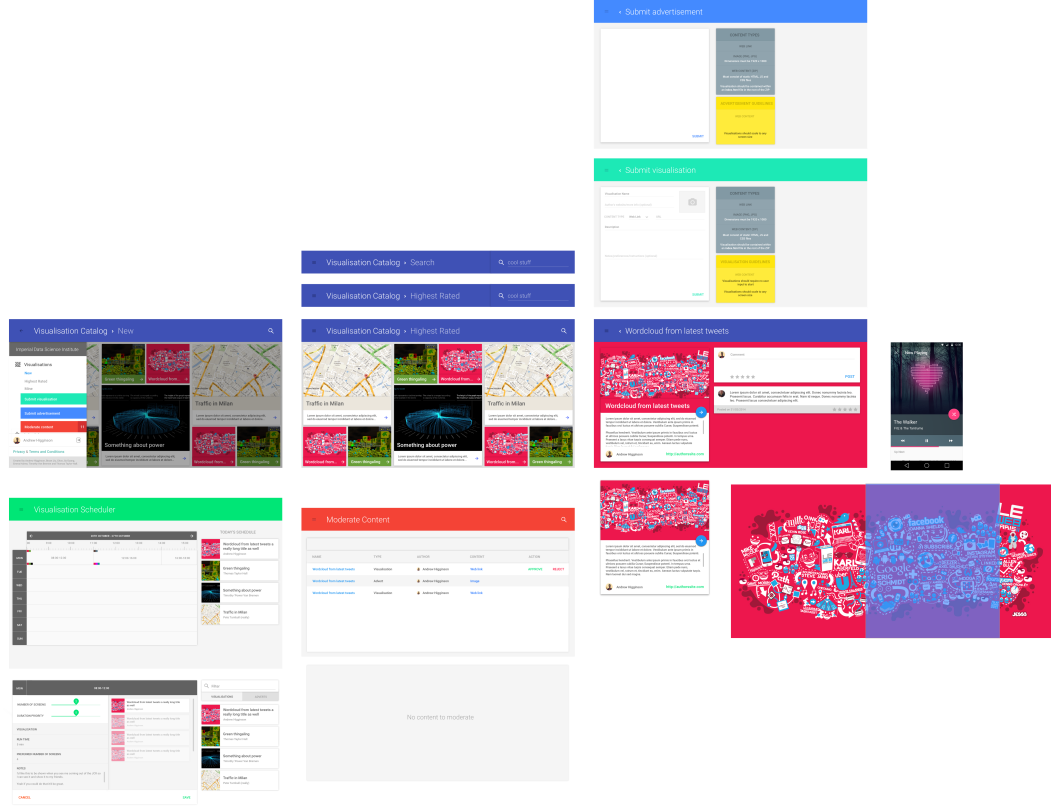
\includegraphics[width = 0.9\textwidth, trim = 0 0 0 0cm, clip]{./eval/mockup.png}
   \end{center}
   \caption{Mockups on User Interface}
   \label{fig:eval_mockup}
\end{figure}

\subsubsection{Requirements on intangible ideas}

Compared to UIs which users can see and feel, we believed that uncovering the client's assumption on playout scheduling via mockups or prototypes will not be feasible as the scheduling algorithm is mainly rule-based. Instead, we delivered our ideas to our supervisore with whiteboard illustrations, and recorded his feedback.

Throughout these discussions, we uncovered several assumptions made by our supervisor, one of which is expecting the scheduling algorithm to ensure that playout time is directly proportional to metric set by administrators. In response, we have created additional unit tests to incorporate such requirements in our scheduling algorithm.

\begin{figure}[ht]
  \begin{minipage}{0.46\textwidth}
      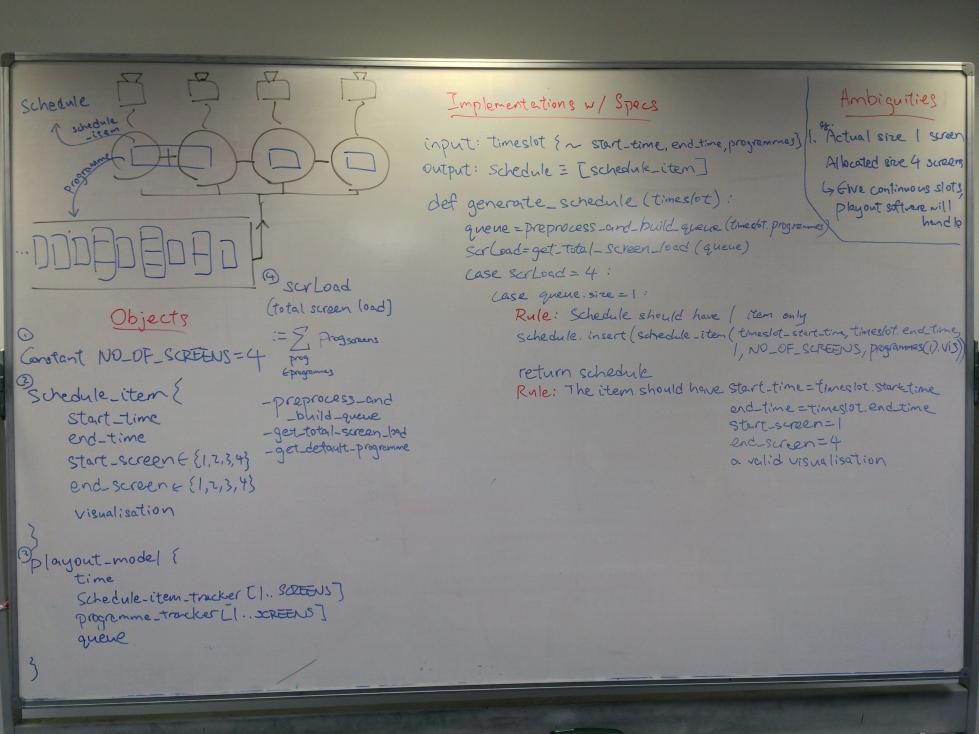
\includegraphics[width = 0.99\textwidth, trim = 0 1cm 0 1.5cm, clip]{./eval/scheduling_whiteboard.jpg}
  \end{minipage}
  \begin{minipage}{0.53\textwidth}
      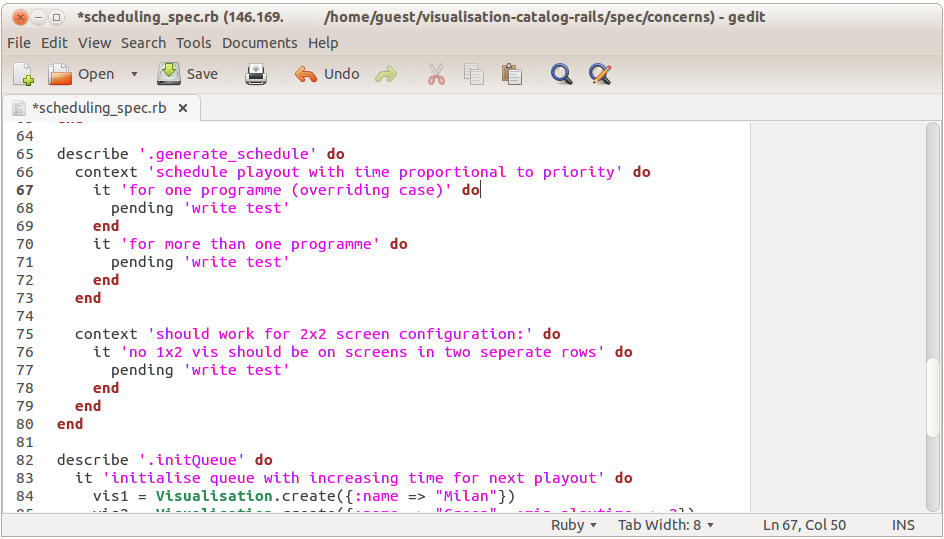
\includegraphics[width = 0.99\textwidth]{./eval/scheduling_spec.png}
  \end{minipage}
  \caption{Capturing scheduling requirements on whiteboard (left), \\ and subsequently via RSpec unit tests (right)}
  \label{fig:eval_scheduling}
\end{figure}

\subsubsection{User testing}

We also conducted implicit user tests during demonstrations of new features, where we asked our supervisor to complete certain tasks with minimal instructions and guidance (e.g. to navigate to the visualisation scheduling page and schedule some visualisations for playout).

Such testing allowed us to learn what is evident to us but obscure to our users. For example, in one of our demonstrations, we observed that our supervisor made multiple pauses when asked to navigate to the moderation and scheduling pages. This indicated that the icon showing the user menu may not be obvious enough to users, and the description for menu items may not be clear enough. Based on such observations, we changed the size of the ``show menu'' button, and also explored the effect of various font colours on the user menu.

We are planning to extend this user testing to include more potential users, especially those that are ranked second in our list of stakeholders, such as staff and students who may use the platform to submit and 
view visualisations.

\subsection{Evaluation}

Even as we are able to evaluate the correctness of our project by unit and system tests after a feature is implemented via RSpec, we still require some other means to test the quality of our features, as well as our group's progress.

\subsubsection{Validated learning \& Pivoting}

As mentioned in Section \ref{sec:eval_validation}, obtaining feedback via mockups, prototypes with representative data and user testing allowed us to 'pivot' many times with minimal reimplementation overhead. It also allows us to identify problems or learn more about the issues that we are trying to solve, before we write large volumes of code which may end up to be not useful. Moreover, this lean approach \textbf{encourages us} to pivot more often, as there is no reason not to do so.

\subsubsection{Project progress}
	
Quantitatively, we evaluated our project by tracking how fast we were ticking off our initial requirements. Using our Trello board and version control system, we can easily see by whom and at what time each feature has been implemented. By combining these with our estimates of the size of each task, we are able to analyse the group's performance via a Cumulative Flow Diagram (Figure \ref{fig:eval_cumuflow}).

\begin{figure}[ht]
  \centering
    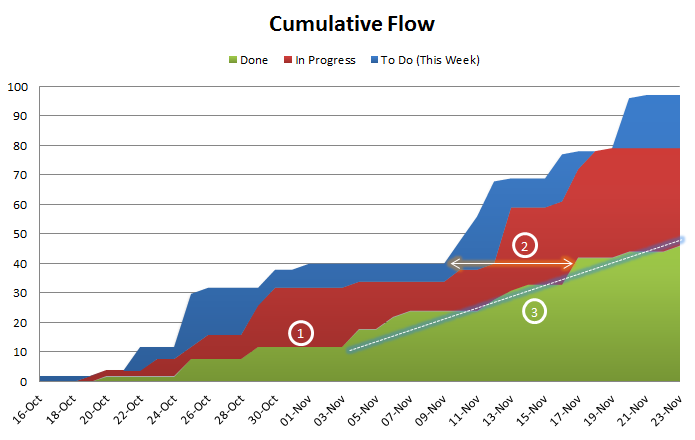
\includegraphics[width = 0.99\textwidth]{./eval/cumu_flow.png}
  \caption{Cumulative flow diagram for our team based on tasks' status}
  \label{fig:eval_cumuflow}
\end{figure}

The diagram tracks the tasks on the columns ``To Do (This week)", ``In Progress" and ``Done", where each task carries a story point based on their size estimate. From the diagram, we can make the following observations:

\begin{enumerate}

  \item In the last week of October, the group did not make much headway for in-progress and to-do tasks. This observation is attributed to problems in setting up Jenkins, which caused a bottleneck in the entire development process.

  \item The lead time (time required between starting and completing a task) is usually around 2 weeks. Given the way we work on a new feature (2 cycles per feature - detailed in Section \ref{sec:uimockup}), we believe that we are making healthy progress in getting individual components of our project done.

  \item Within the first 3 weeks in November, the team has completed tasks worth 35-40 story points. Given that the minimal system is estimated to be worth $\approx$90 story points, we believe that we will be able to meet our deadline in the second week of December with a similar effort.

\end{enumerate}


\newpage
\section{Conclusion}

\subsection{Future Extensions}
TODO:

% ======================================
% ======================================
% ======================================

% -- Appendix
\newpage
\appendix

% -- Initial Spec
\section{(Initial) Specification for Visualisation Wall AppStore}

\textbf{\Large Introduction}

As part of the improvement plan in William Penney Building, windows facing the walkway will be replaced by floor-ceiling glass and projectors that will be internally mounted in WP (similar to that in DoC Teaching Lab). An AppStore system is required to accept upload from various parties and schedule them for playout, subject to moderation.\\

\textbf{\Large System Requirements} \vspace{5pt}

\textbf{\large General}

The system should interact with the following two type of personnel:

\begin{itemize}
  \item General user - who are allowed to submit scientific visualisation and/or advertisements, as well as to state preference on playout.
  \item Administrator - who are allowed to moderate submitted items and to set/override schedules for playout.
\end{itemize}

User hierarchy is not required, it is expected there will be not more than 2 administrators.\\

\textbf{\large Visualisation Submission}

The system should:

\begin{itemize}
\item Accept scientific visualisation, advertising material, events to be advertised (or equivalents) as uploads
\item (Minimally) accept uploads from parties with college login (inc. students, staff, societies)
\item (Ideally) accept uploads from the public (provided external parties has requested and given access to submission)
\item (Minimally) accept submissions of the format: JPEG/BMP/PDF Provide a combination of college login system and access request system as authentication/ authorisation
\item Host data in an internal (provided) cloudstack\\
\end{itemize}

\textbf{\large Moderation}

The system should allow administrators to moderate submitted visualisations (et. al.) - to approve or disapprove submissions.\\

\textbf{\large Scheduling and Playout}

The scheduling system should:

\begin{itemize}
\item Schedule items to play out in rotation (no requirement on scheduling algorithms)
\item Schedule scientific visualisation to play longer than advertisements (or equivalents)
\item Provide administrators ability to control visualisation scheduling (manual scheduling is expected to be conducted on weekly basis)
\item (Prefered) provide administrators options to override scheduled playouts - e.g. to display a specified item on top of other visualisations
\item Allow user to specify visualisation preference (but without control of schedules)
\end{itemize}

The playout system would comprise of:

\begin{itemize}
\item 4 HD Projected Screen - Landscape orientation (4:3 aspect ratio) - controlled by one machine 
\item (Optional) 84” 4K Multi-touch screen - controlled by another machine
\end{itemize}

The playout system would:

\begin{itemize}
\item Size visualisation (or equivalents) automatically (e.g. scale fluidly) (Highly possibly) be web-based and playout via browsers
\item Be run from 8am - 8pm (but should be built to run arbitrary hours)
\item Be scalable in projecting on screens (e.g. 4x1 or 2x2 configuration)\\
\end{itemize}

\textbf{\large Security}

The system should be secure from external interference, especially for playouts.\\

\textbf{\large Miscellaneous}

\begin{itemize}
\item The system should provide an RESTful API for third-party upload/ playout.
Development standards/requirements are welcomed for visualisation, but should be kept minimal for general web pages be shown
\item The system should be branded under Imperial’s Data Science Institute\\
\end{itemize}


\textbf{\Large Available Technologies/ Resources} \vspace{5pt}

\textbf{\large 4x HD Projection Screen}

Screens are controlled by a single, custom machine with graphics card via HDMI cables. It is believed that Windows provide better driver support yet it is fine to run on Linux as long as Chrome is able to be run.\\

\textbf{\large 84” 4K Multi-touch Screen}

The multi-touch screen is run by a dedicated machine in Windows, which the touch screen driver is based on.\\

\textbf{\large Cloudstack/ Virtual Machine}

The system is expected to run on a virtual cloudstack. Virtual machine preinstalled with Windows Server 2008/ Linux Server is available with SQL Instances, Python, PHP, etc. VM can be access remotely (e.g. via linux kernel).\\
% ---

\end{document}